%% 
%% Copyright 2007, 2008, 2009 Elsevier Ltd
%% 
%% This file is part of the 'Elsarticle Bundle'.
%% ---------------------------------------------
%% 
%% It may be distributed under the conditions of the LaTeX Project Public
%% License, either version 1.2 of this license or (at your option) any
%% later version.  The latest version of this license is in
%%    http://www.latex-project.org/lppl.txt
%% and version 1.2 or later is part of all distributions of LaTeX
%% version 1999/12/01 or later.
%% 
%% The list of all files belonging to the 'Elsarticle Bundle' is
%% given in the file `manifest.txt'.
%% 
%% Template article for Elsevier's document class `elsarticle'
%% with harvard style bibliographic references
%% SP 2008/03/01

%\documentclass[preprint,12pt,authoryear]{elsarticle}  %default in the template
%\documentclass[preprint,10pt,authoryear]{elsarticle}

%% Use the option review to obtain double line spacing
%% \documentclass[authoryear,preprint,review,12pt]{elsarticle}

%% Use the options 1p,twocolumn; 3p; 3p,twocolumn; 5p; or 5p,twocolumn
%% for a journal layout:
%% \documentclass[final,1p,times,authoryear]{elsarticle}
%% \documentclass[final,1p,times,twocolumn,authoryear]{elsarticle}
 \documentclass[final,3p,times,authoryear]{elsarticle}
%% \documentclass[final,3p,times,twocolumn,authoryear]{elsarticle}
%% \documentclass[final,5p,times,authoryear]{elsarticle}
%% \documentclass[final,5p,times,twocolumn,authoryear]{elsarticle}

%% For including figures, graphicx.sty has been loaded in
%% elsarticle.cls. If you prefer to use the old commands
%% please give \usepackage{epsfig}

%% The amssymb package provides various useful mathematical symbols
\usepackage{amssymb}
%% The amsthm package provides extended theorem environments
 \usepackage{amsthm}
 \usepackage{amsmath}
 \usepackage{color}
 \usepackage{amsmath}
\usepackage{siunitx}


\usepackage{framed} % Framing content
\usepackage{multicol} % Multiple columns environment
\usepackage{nomencl} % Nomenclature package
\makenomenclature
%\setlength{\nomitemsep}{-\parskip} % Baseline skip between items
\setlength{\nomitemsep}{0.01cm}
\renewcommand*\nompreamble{\begin{multicols}{2}}
\renewcommand*\nompostamble{\end{multicols}}
\newcommand{\degreeC}{\ensuremath{^\circ}C }

\usepackage[nonumberlist]{glossaries}
\makeglossaries 


%% The lineno packages adds line numbers. Start line numbering with
%% \begin{linenumbers}, end it with \end{linenumbers}. Or switch it on
%% for the whole article with \linenumbers.
%% \usepackage{lineno}

\journal{Urban Climate}


\begin{document}


\newglossaryentry{Tmrt}{name={$T_{mrt}$},symbol={\ensuremath{T_{mrt}}},description={mean radiant temperature (\SI{}{\degreeCelsius}}}
\newglossaryentry{UTCI}{name={$UTCI$},symbol={\ensuremath{UTCI}},description={universal thermal climate index}}
\newglossaryentry{Tsurf}{name={$T_{surf}$},symbol={\ensuremath{T_{surf}}},description={surface temperature from the force-restore model (\degreeC)}}
\newglossaryentry{Tg}{name={\ensuremath{T_{g}}},symbol={\ensuremath{T_{g}}},description={globe temperature (K)}}
\newglossaryentry{Tcan}{name={\ensuremath{T_{can}}},symbol={\ensuremath{T_{can}}},description={canopy air temperature (z < z$_{H}$) (K)}} 
\newglossaryentry{A}{name={\ensuremath{A}},symbol={\ensuremath{A}},description={surface area of a sphere of diameter $D$, of value 0.15m}}
\newglossaryentry{D}{name={\ensuremath{D}},symbol={\ensuremath{D}},description={diameter of sphere (m)}}
\newglossaryentry{Nu}{name={\ensuremath{Nu}},symbol={\ensuremath{Nu}},description={Nusselt number (-)}}
\newglossaryentry{Re}{name={\ensuremath{Re}},symbol={\ensuremath{Re}},description={Reynolds number (-)}}
\newglossaryentry{Pr}{name={\ensuremath{Pr}},symbol={\ensuremath{Pr}},description={Prandtl number (-)}}
\newglossaryentry{k}{name={\ensuremath{k}},symbol={\ensuremath{k}},description={thermal conductivity of the fluid (i.e. air) (W m$^{-1}$ K$^{-1}$)}}
\newglossaryentry{Tsfc}{name={\ensuremath{T_{sfc}}},symbol={\ensuremath{T_{sfc}}},description={surface temperature (K)}} 




%
%
%
%
%%\newglossaryentry{E}{name={\ensuremath{E}},symbol={\ensuremath{E}},description={net evapotranspiration}} 
%\newglossaryentry{culdesac}{name=cul-de-sac,description={passage or street closed at one end}}
%\newglossaryentry{Tmrt}{name=\ensuremath{T\textsubscript{mrt}},symbol=\ensuremath{T\textsubscript{mrt}},description={mean radiant temperature (\degreeC)}}
%\newglossaryentry{ohm}{name=ohm,symbol={\ensuremath{\Omega}},description=unit of electrical resistance}
%\newglossaryentry{kup}{name=\ensuremath{K\uparrow},symbol=\ensuremath{{K\uparrow}},description={upward shortwave radiative flux density (W m$^{-2}$)}}
%\newglossaryentry{kdown}{name=\ensuremath{K\downarrow},symbol=\ensuremath{{K\downarrow}},description={downward shortwave radiative flux density (W m$^{-2}$)}}
\newglossaryentry{lup}{name=\ensuremath{L\uparrow},symbol=\ensuremath{{L\uparrow}},description={upward longwave radiative flux density (W m$^{-2}$)}}
\newglossaryentry{ldown}{name=\ensuremath{L\downarrow},symbol=\ensuremath{{L\downarrow}},description={downward longwave radiative flux density (W m$^{-2}$)}}
%\newglossaryentry{q*}{name=\ensuremath{Q^{*}},symbol=\ensuremath{{Q^{*}}},description={net radiation flux density (W m$^{-2}$)}}
%\newglossaryentry{q*pre}{name=\ensuremath{Q^{*}_{pre}},symbol=\ensuremath{{Q^{*}_{pre}}},description={preliminary calculation of net radiation flux density (W m$^{-2}$)}}
%\newglossaryentry{q*veg}{name=\ensuremath{Q^{*}_{veg}},symbol=\ensuremath{{Q^{*}_{veg}}},description={calculation of vegetation net radiation flux density (W m$^{-2}$)}}
%\newglossaryentry{qf}{name={\ensuremath{Q\textsubscript{F}}},symbol={\ensuremath{Q\textsubscript{F}}},description={anthropogenic heat (W m$^{-2}$)}}
%\newglossaryentry{qh}{name={\ensuremath{Q\textsubscript{H}}},symbol={\ensuremath{Q\textsubscript{H}}},description={sensible heat flux (W m$^{-2}$)}}
%\newglossaryentry{qhveg}{name={\ensuremath{Q\textsubscript{H,veg}}},symbol={\ensuremath{Q\textsubscript{H,veg}}},description={calculation of vegetation sensible heat flux (W m$^{-2}$)}}
%\newglossaryentry{qe}{name={\ensuremath{Q\textsubscript{E}}},symbol={\ensuremath{Q\textsubscript{E}}},description={latent heat flux (W m$^{-2}$)}}
%\newglossaryentry{qg}{name={\ensuremath{Q\textsubscript{G}}},symbol={\ensuremath{Q\textsubscript{G}}},description={ground heat storage (W m$^{-2}$)}}
%\newglossaryentry{qgveg}{name={\ensuremath{Q\textsubscript{G,veg}}},symbol={\ensuremath{Q\textsubscript{G,veg}}},description={calculation of vegetation ground heat storage (W m$^{-2}$)}}
%\newglossaryentry{qgstreet}{name={\ensuremath{Q\textsubscript{G,street}}},symbol={\ensuremath{Q\textsubscript{G,street}}},description={calculation of street ground heat storage (W m$^{-2}$)}}
%\newglossaryentry{qeveg}{name={\ensuremath{Q\textsubscript{E,veg}}},symbol={\ensuremath{Q\textsubscript{E,veg}}},description={calculation of vegetation latent heat flux (W m$^{-2}$)}}
%\newglossaryentry{qemaespa}{name={\ensuremath{Q\textsubscript{E,MAESPA}}},symbol={\ensuremath{Q\textsubscript{E,MAESPA}}},description={MAESPA calculation of vegetation latent heat flux (W m$^{-2}$)}}
%\newglossaryentry{qgl}{name={\ensuremath{Q\textsubscript{Gl}}},symbol={\ensuremath{Q\textsubscript{Gl}}},description={global radiation (solar + downward thermal) (W m$^{-2}$)}}
%\newglossaryentry{ql}{name={\ensuremath{Q\textsubscript{L}}},symbol={\ensuremath{Q\textsubscript{L}}},description={longwave radiation (W m$^{-2}$)}}
%\newglossaryentry{qc}{name={\ensuremath{Q\textsubscript{C}}},symbol={\ensuremath{Q\textsubscript{C}}},description={soil heat transport (to deeper soil layers) (W m$^{-2}$)}}
%\newglossaryentry{qs}{name={\ensuremath{\Delta Q\textsubscript{S}}},symbol={\ensuremath{\Delta Q\textsubscript{S}}},description={storage heat flux density (volume) (W m$^{-2}$)}}
%\newglossaryentry{qa}{name={\ensuremath{\Delta Q\textsubscript{A}}},symbol={\ensuremath{\Delta Q\textsubscript{A}}},description={net advective (horizontal air movement) heat flux (W m$^{-2}$)}} 
%\newglossaryentry{p}{name={\ensuremath{P}},symbol={\ensuremath{P}},description={precipitation (mm)}} 
%\newglossaryentry{F}{name={\ensuremath{F}},symbol={\ensuremath{F}},description={moisture release by combustion (mm, kg m$^{-2}$s$^{-1}$)}}  
%\newglossaryentry{I}{name={\ensuremath{I}},symbol={\ensuremath{I}},description={piped water supply per unit horizontal area (mm, kg m$^{-2}$s$^{-1}$)}} 
%\newglossaryentry{E}{name={\ensuremath{E}},symbol={\ensuremath{E}},description={evapotranspiration (mm, kg m$^{-2}$s$^{-1}$)}} 
%\newglossaryentry{deltar}{name={\ensuremath{\Delta r}},symbol={\ensuremath{\Delta r}},description={net run-off (mm, kg m$^{-2}$s$^{-1}$)}} 
%\newglossaryentry{deltaS}{name={\ensuremath{\Delta S}},symbol={\ensuremath{\Delta S}},description={net moisture storage (kg; kg m$^{-3}$s$^{-1}$)}} 
%\newglossaryentry{deltaA}{name={\ensuremath{\Delta A}},symbol={\ensuremath{\Delta A}},description={net moisture advection (kg; kg m$^{-3}$s$^{-1}$)}}
%\newglossaryentry{H}{name={\ensuremath{H}},symbol={\ensuremath{H}},description={internal body heat production (W m$^{-2}$)}}
%\newglossaryentry{Ed}{name={\ensuremath{E\textsubscript{d}}},symbol={\ensuremath{E\textsubscript{d}}},description={heat loss through water evaporation from the skin (W m$^{-2}$)}}
%\newglossaryentry{Esw}{name={\ensuremath{E\textsubscript{sw}}},symbol={\ensuremath{E\textsubscript{sw}}},description={heat loss through sweating (W m$^{-2}$)}}
%\newglossaryentry{Ere}{name={\ensuremath{E\textsubscript{re}}},symbol={\ensuremath{E\textsubscript{re}}},description={heat loss through respiration (W m$^{-2}$)}}
%\newglossaryentry{L}{name={\ensuremath{L}},symbol={\ensuremath{L}},description={dry respiration heat loss (W m$^{-2}$)}}
%\newglossaryentry{R}{name={\ensuremath{R}},symbol={\ensuremath{R}},description={heat loss by radiation from the surface of a clothed body (W m$^{-2}$)}}
%\newglossaryentry{C}{name={\ensuremath{C}},symbol={\ensuremath{C}},description={heat loss through convection from the surface of a clothed body (W m$^{-2}$)}}
%\newglossaryentry{Pa}{name={\ensuremath{P\textsubscript{a}}},symbol={\ensuremath{P\textsubscript{a}}},description={partial vapour pressure (Pa)}}
\newglossaryentry{Ta}{name={\ensuremath{T\textsubscript{a}}},symbol={\ensuremath{T\textsubscript{a}}},description={dry bulb air temperature (K)}}
%\newglossaryentry{Tcl}{name={\ensuremath{T\textsubscript{cl}}},symbol={\ensuremath{T\textsubscript{cl}}},description={clothing surface temperature}}
%\newglossaryentry{PET}{name={\ensuremath{PET}},symbol={\ensuremath{PET}},description={Physiological Equivalent Temperature}}
%\newglossaryentry{rho}{name={\ensuremath{\rho}},symbol={\ensuremath{\rho}},description={(temperature-dependent) density of air (=1.2 kg m$^{-2}$)}}
%\newglossaryentry{To}{name={\ensuremath{T_{o}}},symbol={\ensuremath{T_{o}}},description={temperature (K)}}
%\newglossaryentry{qo}{name={\ensuremath{q_{o}}},symbol={\ensuremath{q_{o}}},description={surface humidity (kg kg$^{-1}$)}}
%\newglossaryentry{Eo}{name={\ensuremath{E_{o}}},symbol={\ensuremath{E_{o}}},description={surface vapour pressure (Pa)}}
%\newglossaryentry{rst}{name={\ensuremath{r_{st}}},symbol={\ensuremath{r_{st}}},description={effective surface resistance of the leaves (s m$^{-1}$)}}
%\newglossaryentry{rsti}{name={\ensuremath{r_{sti}}},symbol={\ensuremath{r_{sti}}},description={effective surface resistance of the leaves of ith area (s m$^{-1}$)}}
%\newglossaryentry{LAi}{name={\ensuremath{L_{A,i}}},symbol={\ensuremath{L_{A,i}}},description={area of the ith leaf over ground area (m$^{2}$)}}
%\newglossaryentry{A}{name={\ensuremath{A}},symbol={\ensuremath{A}},description={ground area (m$^{2}$)}}
%\newglossaryentry{LAI}{name={\ensuremath{LAI}},symbol={\ensuremath{LAI}},description={leaf area index (m$^{2}$ m$^{-2}$)}}
%\newglossaryentry{aleaf}{name={\ensuremath{A_{leaf}}},symbol={\ensuremath{A_{leaf}}},description={total leaf area (m$^{2}$)}}
%
%
%
%\newglossaryentry{cair,H}{name={\ensuremath{c_{air,H}}},symbol={\ensuremath{c_{air,H}}},description={average heat capacity per unit plan area of air below z$_{H}$ (J m$^{-2}$K$^{-1}$)}} 
%\newglossaryentry{C_}{name={\ensuremath{C}},symbol={\ensuremath{C}},description={volumetric heat capacities (J m$^{-3}$K$^{-1}$)}} 
%\newglossaryentry{ea}{name={\ensuremath{e_{a}}},symbol={\ensuremath{e_{a}}},description={water vapour pressure at z$_{ref}$ (hPa)}} 
%\newglossaryentry{G}{name={\ensuremath{G}},symbol={\ensuremath{G}},description={conductive heat flux density (W m$^{-2}$)}} 
%\newglossaryentry{H/W}{name={\ensuremath{H/W}},symbol={\ensuremath{H/W}},description={mean building-height-to-street-width ratio of canyon or regular cube array}} 
%\newglossaryentry{H-W3D}{name={\ensuremath{H/W3D}},symbol={\ensuremath{H/W3D}},description={mean wall-to-street area ratio of regular cube arrays}} 
%\newglossaryentry{Hcan}{name={\ensuremath{H_{can}}},symbol={\ensuremath{H_{can}}},description={summed canopy patch convective sensible heat fluxes per canopy plan area (W m$^{-2}$)}} 
\newglossaryentry{h}{name={\ensuremath{h}},symbol={\ensuremath{h}},description={convective heat transfer coefficient for flow around a sphere (W m$^{-2}$K$^{-1}$)}} 
%\newglossaryentry{H_}{name={\ensuremath{H}},symbol={\ensuremath{H}},description={convective sensible heat flux density (W m$^{-2}$)}} 
%\newglossaryentry{htop}{name={\ensuremath{h_{top}}},symbol={\ensuremath{h_{top}}},description={convective heat transfer coefficient between canopy air and boundary layer (W m$^{-2}$K$^{-1}$)}} 
%\newglossaryentry{Htop}{name={\ensuremath{H_{top}}},symbol={\ensuremath{H_{top}}},description={convective sensible heat flux density between canopy air and boundary layer (W m$^{-2}$)}} 
%\newglossaryentry{i, j}{name={\ensuremath{i, j}},symbol={\ensuremath{i, j}},description={patch index/number k thermal conductivity,W m$^{-1}$K$^{-1}$}} 
%\newglossaryentry{K↑}{name={\ensuremath{K↑}},symbol={\ensuremath{K↑}},description={upward shortwave radiative flux density (W m$^{-2}$)}} 
%\newglossaryentry{K↓dif}{name={\ensuremath{K↓dif}},symbol={\ensuremath{K↓dif}},description={incident diffuse shortwave flux density (W m$^{-2}$)}} 
%\newglossaryentry{K↓dir}{name={\ensuremath{K↓dir}},symbol={\ensuremath{K↓dir}},description={incident direct shortwave flux density (W m$^{-2}$)}} 
%\newglossaryentry{K↓i}{name={\ensuremath{K↓i}},symbol={\ensuremath{K↓i}},description={incident shortwave radiative flux density at patch i after multiple reflections (W m$^{-2}$)}} 
%\newglossaryentry{K↑i}{name={\ensuremath{K↑i}},symbol={\ensuremath{K↑i}},description={reflected shortwave radiative flux density at patch i after multiple reflections (W m$^{-2}$)}} 
%\newglossaryentry{Lh}{name={\ensuremath{Lh}},symbol={\ensuremath{Lh}},description={forcing height for patch convection,m}} 
%\newglossaryentry{lp}{name={\ensuremath{l_{p}}},symbol={\ensuremath{l_{p}}},description={length of a patch side (m)}} 
%\newglossaryentry{LR}{name={\ensuremath{LR}},symbol={\ensuremath{LR}},description={average roof length,m}} 
%\newglossaryentry{L↑}{name={\ensuremath{L↑}},symbol={\ensuremath{L↑}},description={upward longwave radiative flux density (W m$^{-2}$)}} 
%\newglossaryentry{L↓}{name={\ensuremath{L↓}},symbol={\ensuremath{L↓}},description={downward longwave flux density from the sky (W m$^{-2}$)}} 
%\newglossaryentry{L↓i}{name={\ensuremath{L↓i}},symbol={\ensuremath{L↓i}},description={incident longwave flux density at patch i after multiple reflections, W m$^{-2}$}} 
%\newglossaryentry{m}{name={\ensuremath{m}},symbol={\ensuremath{m}},description={timestep index}} 
%\newglossaryentry{n}{name={\ensuremath{n}},symbol={\ensuremath{n}},description={total number of patches}}
%\newglossaryentry{p_}{name={\ensuremath{p}},symbol={\ensuremath{p}},description={number of layers in a patch (conduction)}} 
%\newglossaryentry{Pa_}{name={\ensuremath{Pa}},symbol={\ensuremath{Pa}},description={atmospheric pressure at zref (hPa)}} 
%\newglossaryentry{Q∗}{name={\ensuremath{Q∗}},symbol={\ensuremath{Q∗}},description={net radiation flux density (W m$^{-2}$)}} 
%\newglossaryentry{Qh}{name={\ensuremath{Q_{H}}},symbol={\ensuremath{Q_{H}}},description={convective sensible heat flux density (volume) (W m$^{-2}$)}} 
%\newglossaryentry{q}{name={\ensuremath{q}},symbol={\ensuremath{q}},description={reflection number}} 
%\newglossaryentry{Rq}{name={\ensuremath{Rq}},symbol={\ensuremath{Rq}},description={reflected radiative flux density (solar or longwave) at reflection q (W m$^{-2}$)}} 
%\newglossaryentry{rw}{name={\ensuremath{r_{w}}},symbol={\ensuremath{r_{w}}},description={wall roughness coefficient}} 
%\newglossaryentry{rwi}{name={\ensuremath{r_{w,i}}},symbol={\ensuremath{r_{w,i}}},description={wall roughness coefficient of patch i}} 
%\newglossaryentry{Sd}{name={\ensuremath{Sd}},symbol={\ensuremath{Sd}},description={refers to the sub-domain}} 
%\newglossaryentry{T(z)}{name={\ensuremath{T(z)}},symbol={\ensuremath{T(z)}},description={air temperature at height z (K)}} 
%\newglossaryentry{Ta_}{name={\ensuremath{T_{a}}},symbol={\ensuremath{T_{a}}},description={air temperature at z$_{ref}$ (K)}} 
%\newglossaryentry{Tapp}{name={\ensuremath{T_{app}}},symbol={\ensuremath{T_{app}}},description={apparent surface temperature (K)}} 
%\newglossaryentry{Tb (b = 1, ... ,p)}{name={\ensuremath{Tb (b = 1, ... ,p}},symbol={\ensuremath{Tb (b = 1, ... ,p}},description={substrate layer temperatures (K) }} 
%\newglossaryentry{Tcan}{name={\ensuremath{T_{can}}},symbol={\ensuremath{T_{can}}},description={canopy air temperature (z < z$_{H}$) (K)}} 
%\newglossaryentry{TD}{name={\ensuremath{T_{D}}},symbol={\ensuremath{T_{D}}},description={deep-soil temperature (K)}} 
%\newglossaryentry{TINT}{name={\ensuremath{T_{INT}}},symbol={\ensuremath{T_{INT}}},description={building internal temperature (K)}} 
%\newglossaryentry{Tlog(z)}{name={\ensuremath{T_{log}(z)}},symbol={\ensuremath{T_{log}(z)}},description={air temperature profile above z$_{H}$ (K)}} 
%\newglossaryentry{TR}{name={\ensuremath{T_{R}}},symbol={\ensuremath{T_{R}}},description={mean roof surface temperature (K)}} 
%\newglossaryentry{Tr}{name={\ensuremath{T_{r}}},symbol={\ensuremath{T_{r}}},description={mean road surface temperature (K)}} 
%\newglossaryentry{Tsfc}{name={\ensuremath{T\textsubscript{sfc}}},symbol={\ensuremath{T\textsubscript{sfc}}},description={surface temperature (K)}} 
%\newglossaryentry{Tsfci}{name={\ensuremath{T\textsubscript{sfc,i}}},symbol={\ensuremath{T\textsubscript{sfc,i}}},description={surface temperature of patch i (K)}} 
%\newglossaryentry{Tsfcveg}{name={\ensuremath{T_{sfc,veg}}},symbol={\ensuremath{T_{sfc,veg}}},description={vegetation surface temperature (K)}} 
%\newglossaryentry{TW}{name={\ensuremath{T_{W}}},symbol={\ensuremath{T_{W}}},description={mean wall surface temperature (K)}} 
%\newglossaryentry{U(z)}{name={\ensuremath{U(z)}},symbol={\ensuremath{U(z)}},description={wind speed at height z (m s$^{-1}$)}} 
%\newglossaryentry{Ua}{name={\ensuremath{U_{a}}},symbol={\ensuremath{U_{a}}},description={wind speed at z$_{ref}$ (m s$^{-1}$)}} 
%\newglossaryentry{Ueff(z)}{name={\ensuremath{U_{eff}(z)}},symbol={\ensuremath{U_{eff}(z)}},description={effective wind speed at height z (m s$^{-1}$)}} 
%\newglossaryentry{x, y, z}{name={\ensuremath{x, y, z}},symbol={\ensuremath{x, y, z}},description={location in space}} 
%\newglossaryentry{xL}{name={\ensuremath{x_{L}}},symbol={\ensuremath{x_{L}}},description={building width (m)}} 
%\newglossaryentry{xW}{name={\ensuremath{x_{W}}},symbol={\ensuremath{x_{W}}},description={canyon (street) width (m)}} 
%\newglossaryentry{z0h}{name={\ensuremath{z_{0h}}},symbol={\ensuremath{z_{0h}}},description={roughness length for heat (m)}} 
%\newglossaryentry{z0m}{name={\ensuremath{z_{0m}}},symbol={\ensuremath{z_{0m}}},description={roughness length for momentum (patch) (m)}} 
%\newglossaryentry{z0}{name={\ensuremath{z_{0}}},symbol={\ensuremath{z_{0}}},description={roughness length (m)}} 
%\newglossaryentry{z0town}{name={\ensuremath{z_{0town}}},symbol={\ensuremath{z_{0town}}},description={roughness length for momentum (domain) (m)}} 
%\newglossaryentry{zd}{name={\ensuremath{z_{D}}},symbol={\ensuremath{z_{D}}},description={displacement height (m)}} 
%\newglossaryentry{zH}{name={\ensuremath{z_{H}}},symbol={\ensuremath{z_{H}}},description={mean building height (m)}} 
%\newglossaryentry{zh}{name={\ensuremath{z_{H}}},symbol={\ensuremath{z_{H}}},description={measurement height of wind speed (m)}} 
%\newglossaryentry{zht}{name={\ensuremath{z_{Ht}}},symbol={\ensuremath{z_{Ht}}},description={measurement height of wind speed (m)}} 
%\newglossaryentry{zpd}{name={\ensuremath{z_{PD}}},symbol={\ensuremath{z_{PD}}},description={zero-plane displacement height (m)}} 
%\newglossaryentry{z0ht}{name={\ensuremath{z_{0,Ht}}},symbol={\ensuremath{z_{0,Ht}}},description={roughness length (m)}} 
%
%
%
%\newglossaryentry{z}{name={\ensuremath{z}},symbol={\ensuremath{z}},description={height in the model domain (m)}} 
%\newglossaryentry{zhorz}{name={\ensuremath{z_{horz}}},symbol={\ensuremath{z_{horz}}},description={height of patch forcing U(z) and T(z) above street level (m)}} 
%\newglossaryentry{zhorzi}{name={\ensuremath{z_{horz,i}}},symbol={\ensuremath{z_{horz,i}}},description={height of patch forcing U(z) and T(z) above street level of patch i (m)}} 
%\newglossaryentry{zref}{name={\ensuremath{z_{ref}}},symbol={\ensuremath{z_{ref}}},description={reference height for forcing data (m)}} 
%\newglossaryentry{alpha}{name={\ensuremath{\alpha}},symbol={\ensuremath{\alpha}},description={shortwave albedo}} 
%\newglossaryentry{alphar}{name={\ensuremath{\alpha r}},symbol={\ensuremath{\alpha r}},description={shortwave albedo of streets}} 
%\newglossaryentry{alphaR}{name={\ensuremath{\alpha R}},symbol={\ensuremath{\alpha R}},description={shortwave albedo of roofs}} 
%\newglossaryentry{alphaW}{name={\ensuremath{\alpha W}},symbol={\ensuremath{\alpha W}},description={shortwave albedo of walls}} 
% 
%\newglossaryentry{deltaαD}{name={\ensuremath{\deltaαD}},symbol={\ensuremath{\deltaαD}},description={sub-domain albedo change threshold}} 
%\newglossaryentry{deltaQs}{name={\ensuremath{\Delta Qs}},symbol={\ensuremath{\Delta Qs}},description={storage heat flux density (volume) (W m$^{-2}$)}} 
%\newglossaryentry{deltat}{name={\ensuremath{\Delta t}},symbol={\ensuremath{\Delta t}},description={timestep size (s)}} 
%\newglossaryentry{deltaTcrit}{name={\ensuremath{\Delta Tcrit}},symbol={\ensuremath{\Delta Tcrit}},description={surface temperature change threshold (K)}} 
%\newglossaryentry{deltax}{name={\ensuremath{\Delta x}},symbol={\ensuremath{\Delta x}},description={layer thickness (m)}} 
%\newglossaryentry{epsilon}{name={\ensuremath{\epsilon}},symbol={\ensuremath{\epsilon}},description={longwave emissivity}} 
%\newglossaryentry{epsilonr}{name={\ensuremath{\epsilon r}},symbol={\ensuremath{\epsilon r}},description={longwave emissivity of streets}} 
%\newglossaryentry{epsilonR}{name={\ensuremath{\epsilon R}},symbol={\ensuremath{\epsilon R}},description={longwave emissivity of roofs}} 
%\newglossaryentry{epsilonW}{name={\ensuremath{\epsilon W}},symbol={\ensuremath{\epsilon W}},description={longwave emissivity of walls}} 
%
%
%\newglossaryentry{η}{name={\ensuremath{η}},symbol={\ensuremath{η}},description={domain rotation from north (clockwise), ◦}} 
%\newglossaryentry{lambdac}{name={\ensuremath{\lambda_{c}}},symbol={\ensuremath{\lambda_{c}}},description={complete-to-plan area ratio}} 
%\newglossaryentry{lambdaf}{name={\ensuremath{\lambda_{f}}},symbol={\ensuremath{\lambda_{f}}},description={frontal-area-to-plan area ratio}} 
%\newglossaryentry{lambdap}{name={\ensuremath{\lambda_{p}}},symbol={\ensuremath{\lambda_{p}}},description={building-to-plan area ratio}} 
%\newglossaryentry{lambdapH}{name={\ensuremath{\lambda_{ph}}},symbol={\ensuremath{\lambda_{ph}}},description={building-to-plan area ratio at z$_{H}$}} 
\newglossaryentry{sigma}{name={\ensuremath{\sigma}},symbol={\ensuremath{\sigma}},description={Stefan-Boltzmann constant (=5.67 $\times$ 10$^{-8}$ W m$^{-2}$K$^{-4}$)}} 
%\newglossaryentry{ΩINT}{name={\ensuremath{ΩINT}},symbol={\ensuremath{ΩINT}},description={building internal resistance (W m$^{-1}$K$^{-1}$)}} 
%\newglossaryentry{ψi,external}{name={\ensuremath{ψi,external}},symbol={\ensuremath{ψi,external}},description={view factor from a patch i to external surfaces}} 
%\newglossaryentry{ψi,j}{name={\ensuremath{ψi,j}},symbol={\ensuremath{ψi,j}},description={view factor from a patch i to a patch j}} 
%\newglossaryentry{ψi,sky}{name={\ensuremath{ψi,sky}},symbol={\ensuremath{ψi,sky}},description={view factor from a patch i to the sky}} 
%
%\newglossaryentry{RA}{name={\ensuremath{R\textsubscript{A}}},symbol={\ensuremath{R\textsubscript{A}}},description={aerodynamic resistance (s m$^{-1}$)}} 
%\newglossaryentry{RS}{name={\ensuremath{R\textsubscript{S}}},symbol={\ensuremath{R\textsubscript{S}}},description={surface resistance (s m$^{-1}$)}} 
%
%\newglossaryentry{deltaQS}{name={\ensuremath{\Delta Q\textsubscript{S}}},symbol={\ensuremath{\Delta Q\textsubscript{S}}},description={storage heat fluxes (W m$^{-2}$)}} 
%
%\newglossaryentry{ws}{name={\ensuremath{ws}},symbol={\ensuremath{ws}},description={wind speed (m s$^{-1}$)}} 
%\newglossaryentry{rh}{name={\ensuremath{RH}},symbol={\ensuremath{RH}},description={relative humidity (\%)}} 
%\newglossaryentry{epsilonp}{name={\ensuremath{\epsilon _{p}}},symbol={\ensuremath{\epsilon _{p}}},description={emissivity of the human body}} 
%\newglossaryentry{R_}{name={\ensuremath{R}},symbol={\ensuremath{R}},description={ideal gas constant (=8.314 J mol$^{-1}$K$^{-1}$)}} 
%\newglossaryentry{T}{name={\ensuremath{T}},symbol={\ensuremath{T}},description={temperature (K)}} 
%
%\newglossaryentry{deltaHvap}{name={\ensuremath{\Delta H_{vap}}},symbol={\ensuremath{\Delta H_{vap}}},description={enthalpy of evaporation (=42809 J mol$^{-1}$)}} 
%
%
%\newglossaryentry{Po}{name={\ensuremath{P_{o}}},symbol={\ensuremath{P_{o}}},description={vapour pressure of water at infinite temperature (=7.5152 $\times$ 10$^8$ mb)}} 
%\newglossaryentry{Sstr}{name={\ensuremath{S_{str}}},symbol={\ensuremath{S_{str}}},description={mean radiant flux density}} 
%\newglossaryentry{alphak}{name={\ensuremath{\alpha _{k}}},symbol={\ensuremath{\alpha _{k}}},description={absorption coefficient for short-wave radiation}} 
%\newglossaryentry{Hblt}{name={\ensuremath{H _{blt}}},symbol={\ensuremath{H _{blt}}},description={building height (m)}} 
%\newglossaryentry{nhts}{name={\ensuremath{n _{hts}}},symbol={\ensuremath{n _{hts}}},description={number of building heights}} 
%\newglossaryentry{nroofs}{name={\ensuremath{n _{roofs}}},symbol={\ensuremath{n _{roofs}}},description={number of roofs}} 
%\newglossaryentry{diamstem}{name={\ensuremath{diam _{stem}}},symbol={\ensuremath{diam _{stem}}},description={stem diameter (m)}} 
%\newglossaryentry{htrunk}{name={\ensuremath{H _{trunk}}},symbol={\ensuremath{H _{trunk}}},description={trunk height (m)}} 
%\newglossaryentry{hcrown}{name={\ensuremath{H _{crown}}},symbol={\ensuremath{H _{crown}}},description={crown height (m)}} 
%\newglossaryentry{acanopy}{name={\ensuremath{A _{canopy}}},symbol={\ensuremath{A _{canopy}}},description={canopy area ($m^{2}$)}} 
%\newglossaryentry{rcrownx}{name={\ensuremath{r _{x,crown}}},symbol={\ensuremath{r _{x,crown}}},description={crown radius in x direction (m)}} 
%\newglossaryentry{rcrowny}{name={\ensuremath{r _{y,crown}}},symbol={\ensuremath{r _{y,crown}}},description={crown radius in y direction (m)}} 
%
%%\newglossaryentry{et}{name={\ensuremath{et}},symbol={\ensuremath{et}},description={evapotranspiration (mm)}} 
%\newglossaryentry{Amm}{name={\ensuremath{A _{mm}}},symbol={\ensuremath{A _{mm}}},description={2-dimensional tree area (mm$^{2}$)}} 
%\newglossaryentry{Time}{name={\ensuremath{Time}},symbol={\ensuremath{Time}},description={time (seconds)}} 
%
%\newglossaryentry{Atree}{name={\ensuremath{A _{tree}}},symbol={\ensuremath{A _{tree}}},description={2-dimensional tree area (mm$^{2}$)}} 
%\newglossaryentry{alphaveg}{name={\ensuremath{\alpha _{veg}}},symbol={\ensuremath{\alpha _{veg}}},description={shortwave albedo of vegetation}} 
%\newglossaryentry{epsilonveg}{name={\ensuremath{\epsilon _{veg}}},symbol={\ensuremath{\epsilon _{veg}}},description={longwave emissivity of vegetation}} 
%\newglossaryentry{tconv}{name={\ensuremath{T_{conv}}},symbol={\ensuremath{T_{conv}}},description={converging canyon temperature (K)}} 
%\newglossaryentry{hi}{name={\ensuremath{h_{i}}},symbol={\ensuremath{h_{i}}},description={heat transfer coefficient (W m$^{-2}$K$^{-1}$)}} 
%\newglossaryentry{k1}{name={\ensuremath{k_{1}}},symbol={\ensuremath{k_{1}}},description={conversion from pressure units to volumetric units}} 
%\newglossaryentry{T1}{name={\ensuremath{T_{1}}},symbol={\ensuremath{T_{1}}},description={temperature of the shallowest layer (K)}} 
%\newglossaryentry{Tm}{name={\ensuremath{T_{m}}},symbol={\ensuremath{T_{m}}},description={temperature of the deepest layer (K)}} 
%\newglossaryentry{UTCI}{name={\ensuremath{UTCI}},symbol={\ensuremath{UTCI}},description={universal thermal climate index}} 
%\newglossaryentry{ET}{name={\ensuremath{ET}},symbol={\ensuremath{ET}},description={evapotranspiration (mm, kg m$^{-2}$s$^{-1}$)}} 
%\newglossaryentry{d}{ name={\ensuremath{d}}, symbol={\ensuremath{d}}, description={index of agreement (0 <= d <= 1)}} 
%\newglossaryentry{r2}{name={\ensuremath{r^2}},symbol={\ensuremath{r^2}},description={the fraction of variance explained by the model}} 
%\newglossaryentry{rmse}{name={RMSE},symbol={RMSE},description={root mean square error}}
%\newglossaryentry{wsud}{name={WSUD},symbol={WSUD},description={water sensitive urban design}}
%\newglossaryentry{csud}{name={CSUD},symbol={CSUD},description={climate sensitive urban design}}
%\newglossaryentry{htc}{name={HTC},symbol={HTC},description={human thermal comfort}}
%\newglossaryentry{PBM}{name={PBM},symbol={PBM},description={process based model}}
%\newglossaryentry{SEB}{name={SEB},symbol={SEB},description={surface energy balance model}}
%\newglossaryentry{uhi}{name={UHI},symbol={UHI},description={urban heat island}}
%\newglossaryentry{ubl}{name={UBL},symbol={UBL},description={urban boundary layer}}
%\newglossaryentry{PAR}{name={PAR},symbol={PAR},description={photosynthetically active radiation (400 to 700 nm)}}
%\newglossaryentry{NIR}{name={NIR},symbol={NIR},description={near-infrared radiation (700 nm to 2500 nm)}}
%\newglossaryentry{IR}{name={IR},symbol={IR},description={infrared radiation (700 nm to 1mm}}
%
%\newglossaryentry{An}{name={\ensuremath{A_{n}}},symbol={\ensuremath{A_{n}}},description={leaf net assimilation rate ($\mu$mol m$^{-2}$s$^{-1}$)}} 
%\newglossaryentry{gs}{name={\ensuremath{g_{s}}},symbol={\ensuremath{g_{s}}},description={leaf-level stomatal conductance to H$_{2}$O} (mol m$^{-2}$s$^{-1}$)} 
%\newglossaryentry{gs_}{name={\ensuremath{g_{s}}},symbol={\ensuremath{g_{s}}},description={leaf-level stomatal conductance to CO$_{2}$} (mol m$^{-2}$s$^{-1}$)} 
%\newglossaryentry{g0}{name={\ensuremath{g_{0}}},symbol={\ensuremath{g_{0}}},description={conductance when \ensuremath{A_{n}} is zero (mol m$^{-2}$s$^{-1}$)}} 
%\newglossaryentry{g1}{name={\ensuremath{g_{1}}},symbol={\ensuremath{g_{1}}},description={conductance empirical parameter}} 
%\newglossaryentry{Cs}{name={\ensuremath{C_{s}}},symbol={\ensuremath{C_{s}}},description={CO$_{2}$ concentration at the leaf surface ($\mu$mol mol$^{-2}$)}}
%\newglossaryentry{fD}{name={\ensuremath{f(D)}},symbol={\ensuremath{f(D)}},description={function of the leaf-to-air vapour pressure deficit (D)}}
%
%\newglossaryentry{Dpa}{name={\ensuremath{D}},symbol={\ensuremath{D}},description={leaf-to-air vapour pressure deficit (Pa)}}
%\newglossaryentry{D0}{name={\ensuremath{D_{0}}},symbol={\ensuremath{D_{0}}},description={an empirically determined coefficient}}
%
%\newglossaryentry{psiL}{name={\ensuremath{\Psi_{L}}},symbol={\ensuremath{\Psi_{L}}},description={leaf water potential (MPa)}}
%\newglossaryentry{psif}{name={\ensuremath{\Psi_{f}}},symbol={\ensuremath{\Psi_{f}}},description={reference water potential (MPa)}}
%\newglossaryentry{sf}{name={\ensuremath{s_{f}}},symbol={\ensuremath{s_{f}}},description={steepness of the response of \ensuremath{f\Psi_{L}} to \ensuremath{\Psi_{L}}}}
%
%\newglossaryentry{smdeltaA}{name={\ensuremath{\delta{A}}},symbol={\ensuremath{\delta{A}}},description={change in rate of assimilation (mol m$^{-2}$s$^{-1}$)}}
%\newglossaryentry{smdeltaE}{name={\ensuremath{\delta{E}}},symbol={\ensuremath{\delta{E}}},description={change in the rate of transpiration per unit area of leaf (mol m$^{-2}$s$^{-1}$)}}
%
%
%\newglossaryentry{overlineTr}{name={\ensuremath{\overline{T}_{r}}},symbol={\ensuremath{\overline{T}_{r}}},description={mean radiant temperature (K)}}
%\newglossaryentry{TN}{name={\ensuremath{T_{N}}},symbol={\ensuremath{T_{N}}},description={surface temperature of surface N (K)}}
%\newglossaryentry{FpN}{name={\ensuremath{F_{p-N}}},symbol={\ensuremath{F_{p-N}}},description={angle factor between a person and surface N}}
%
%\newglossaryentry{lambdaE}{name={\ensuremath{\lambda E}},symbol={\ensuremath{\lambda E}},description={total latent heat of vaporation (cal g$^{-1}$) }}
%\newglossaryentry{DeltaH}{name={\ensuremath{\Delta H}},symbol={\ensuremath{\Delta H}},description={rate of heat supply (cal cm$^{-2}$sec$^{-1}$)}} 
%\newglossaryentry{rhoC}{name={\ensuremath{\rho c}},symbol={\ensuremath{\rho c}},description={specific heat of air (cal cm$^{-3}$)}} 
%\newglossaryentry{Delta}{name={\ensuremath{\Delta}},symbol={\ensuremath{\Delta}},description={change of saturation vapour pressure with temperature (mb)}} 
%\newglossaryentry{E1}{name={\ensuremath{E_{1}}},symbol={\ensuremath{E_{1}}},description={rate of evaporation from a wet surface with temperature $T\prime$}} 
%\newglossaryentry{E2}{name={\ensuremath{E_{2}}},symbol={\ensuremath{E_{2}}},description={rate of latent heat uptake of water evaporated into saturated air}} 
%\newglossaryentry{gamma}{name={\ensuremath{\gamma}},symbol={\ensuremath{\gamma}},description={latent heat of water (=2.47 $\times$ 10$^{6}$ J kg$^{-1}$)}} 
%\newglossaryentry{D}{name={\ensuremath{D}},symbol={\ensuremath{D}},description={wet-bulb depression}} 
%\newglossaryentry{ra}{name={\ensuremath{r_{a}}},symbol={\ensuremath{r_{a}}},description={time in which 1 cm$^{3}$ of air exchanges heat with 1 cm$^{3}$ of surface}} 
%\newglossaryentry{esT}{name={\ensuremath{e_{s}(T)}},symbol={\ensuremath{e_{s}(T)}},description={saturation vapour pressure at temperature T (Pa)}} 
%\newglossaryentry{e}{name={\ensuremath{e}},symbol={\ensuremath{e}},description={vapour pressure (Pa)}} 
%\newglossaryentry{Ea}{name={\ensuremath{E_{a}}},symbol={\ensuremath{E_{a}}},description={actual evapotranspiration (kg m$^{-2}$s$^{-1}$)}} 
%\newglossaryentry{DeltaS}{name={\ensuremath{\Delta _{S}}},symbol={\ensuremath{\Delta _{S}}},description={slope of the specific humidity/ temperature curve between the air temperature $T_{D}$ and the surface temperature of the vegetation $T_{s}$ (kg kg$^{-1}$ \degreeC)}} 
%\newglossaryentry{a}{name={\ensuremath{A}},symbol={\ensuremath{A}},description={available energy given by A = RN - G (W m$^{-2}$)}} 
%\newglossaryentry{cp}{name={\ensuremath{c_{\rho}}},symbol={\ensuremath{c_{\rho}}},description={specific heat of air at constant pressure (=1.01 $\times$ 10$^{3}$ J kg$^{-1}$ K$^{-1}$)}} 
%
%\newglossaryentry{qwtd}{name={\ensuremath{q_{w},T_{d}}},symbol={\ensuremath{q_{w},T_{d}}},description={saturated specific humidity at dry-bulk temperature, T$_{D}$ (kg kg$^{-1}$)}} 
%\newglossaryentry{qwtdq}{name={\ensuremath{(q_{w},T_{d}-q)}},symbol={\ensuremath{(q_{w},T_{d}-q)}},description={specific humidity deficit (kg kg$^{-1}$)}} 
%\newglossaryentry{r_a}{name={\ensuremath{r_{a}}},symbol={\ensuremath{r_{a}}},description={aerodynamic resistance to the transport of water vapour from the surface to the reference level z (s m$^{-1}$)}} 
%\newglossaryentry{r_c}{name={\ensuremath{r_{c}}},symbol={\ensuremath{r_{c}}},description={(Monteith) canopy resistance to the transport of water from some region within or below the evaporating surface to the surface itself, and is expected to be a function of the stomatal resistance of individual leaves. Under wet-canopy conditions rc = 0 (s m$^{-1}$)}} 
%
%\newglossaryentry{psiisky}{name={\ensuremath{\Psi_{i,sky}}},symbol={\ensuremath{\Psi_{i,sky}}},description={sky view factor of surface patch i}}
%\newglossaryentry{psiij}{name={\ensuremath{\Psi_{i,j}}},symbol={\ensuremath{\Psi_{i,j}}},description={view factor from patch i to patch j}}
%\newglossaryentry{psiexternal}{name={\ensuremath{\Psi_{i,external}}},symbol={\ensuremath{\Psi_{i,external}}},description={view factor from patch i to external surfaces}}
%\newglossaryentry{ldownsky}{name=\ensuremath{L\downarrow_{sky}},symbol=\ensuremath{{L\downarrow_{sky}}},description={domain-level incoming longwave (W m$^{-2}$)}}
%\newglossaryentry{kdowndif}{name=\ensuremath{K\downarrow_{dif}},symbol=\ensuremath{{K\downarrow_{dif}}},description={domain-level incoming diffuse shortwave (W m$^{-2}$)}}
%\newglossaryentry{kdowndir}{name=\ensuremath{K\downarrow_{dir}},symbol=\ensuremath{{K\downarrow_{dir}}},description={domain-level incoming direct shortwave (W m$^{-2}$)}}
%\newglossaryentry{ldownskyi}{name=\ensuremath{L\downarrow_{i,sky}},symbol=\ensuremath{{L\downarrow_{i,sky}}},description={initial incident sky-derived longwave (W m$^{-2}$)}}
%\newglossaryentry{kdowndifi}{name=\ensuremath{K\downarrow_{dif,i}},symbol=\ensuremath{{K\downarrow_{dif,i}}},description={initial incident diffuse shortwave (W m$^{-2}$)}}
%\newglossaryentry{kdowndiri}{name=\ensuremath{K\downarrow_{dir,i}},symbol=\ensuremath{{K\downarrow_{dir,i}}},description={initial incident direct shortwave (W m$^{-2}$)}}
%\newglossaryentry{phi}{name={\ensuremath{\phi}},symbol={\ensuremath{\phi}},description={solar zenith angle (degrees)}} 
%\newglossaryentry{δ}{name={\ensuremath{δ}},symbol={\ensuremath{δ}},description={solar azimuth angle (degrees)}}
%\newglossaryentry{chi}{name={\ensuremath{\chi}},symbol={\ensuremath{\chi}},description={solar zenith angle (degrees)}} 
%\newglossaryentry{chii}{name={\ensuremath{\chi_{i}}},symbol={\ensuremath{\chi_{i}}},description={angle between patch i's normal vector and the vector pointing in the direction of the sun (degrees)}} 
%
%\newglossaryentry{Rqi}{name={\ensuremath{R^{q+1} _{i}}},symbol={\ensuremath{R^{q+1} _{i}}},description={radiation reflected by patch i at reflection q + 1}} 
%\newglossaryentry{Rqj}{name={\ensuremath{R^{q} _{j}}},symbol={\ensuremath{R^{q} _{j}}},description={radiation reflected by patch j at reflection q}} 
%\newglossaryentry{alphai}{name={\ensuremath{\alpha _{i}}},symbol={\ensuremath{\alpha _{i}}},description={shortwave albedo of patch i}}  
%\newglossaryentry{epsiloni}{name={\ensuremath{\epsilon _{i}}},symbol={\ensuremath{\epsilon _{i}}},description={longwave emissivity of patch i}}  
%\newglossaryentry{psiji}{name={\ensuremath{\Psi_{j,i}}},symbol={\ensuremath{\Psi_{j,i}}},description={view factor from patch j to patch i}}
%
%\newglossaryentry{Tb}{name={\ensuremath{T_{b}}},symbol={\ensuremath{T_{b}}},description={temperature of layer b (K)}}
%\newglossaryentry{Cb}{name={\ensuremath{C_{b}}},symbol={\ensuremath{C_{b}}},description={volumetric heat capacity of layer b (J m$^{-2}$K$^{-1}$)}}
%\newglossaryentry{Deltaxb}{name={\ensuremath{\Delta x_{b}}},symbol={\ensuremath{\Delta x_{b}}},description={depth of layer b (m)}}
%\newglossaryentry{gammac}{name={\ensuremath{\gamma}},symbol={\ensuremath{\gamma}},description={degree of implicitness (conduction) (i.e. $\gamma$ = 0 is explicit, $\gamma$ = 1 is implicit)}} 
%\newglossaryentry{Gmbb}{name={\ensuremath{G^{m} _{b,b+1}}},symbol={\ensuremath{G^{m} _{b,b+1}}},description={conductive heat flux between layers b and b + 1 at timestep m (W m$^{-2}$)}}
%\newglossaryentry{F1}{name={\ensuremath{F_{1}}},symbol={\ensuremath{F_{1}}},description={total-area fraction of irradiated leaves on a branch}}
%\newglossaryentry{Hm}{name={\ensuremath{H}},symbol={\ensuremath{H}},description={tree height (m)}}
%\newglossaryentry{RprimeH}{name={\ensuremath{R^{\prime}(h)}},symbol={\ensuremath{R^{\prime}(h)}},description={crown radius at the relative crown height h (m)}}
%\newglossaryentry{hm}{name={\ensuremath{h}},symbol={\ensuremath{h}},description={relative height within the tree crown or the canopy}}
%\newglossaryentry{Bi}{name={\ensuremath{B_{i}}},symbol={\ensuremath{B_{i}}},description={parameters in the leaf area density distributions within the tree crown or canopy (i=1, 2, and 3 for vertical distribution and 4, 5, and 6 for horizontal distribution)}}
%\newglossaryentry{r}{name={\ensuremath{r}},symbol={\ensuremath{r}},description={horizontal distance from the centre of the tree trunk (m)}}
%\newglossaryentry{Ld}{name={\ensuremath{L_{d}}},symbol={\ensuremath{L_{d}}},description={relative leaf area density within the tree crown (m$^{-1}$)}}
%\newglossaryentry{gB}{name={\ensuremath{g_{B}}},symbol={\ensuremath{g_{B}}},description={boundary layer conductance (mol m$^{-2}$s$^{-1}$)}}
%\newglossaryentry{gV}{name={\ensuremath{g_{V}}},symbol={\ensuremath{g_{V}}},description={total conductance to water vapour (mol m$^{-2}$s$^{-1}$)}}
%\newglossaryentry{gC}{name={\ensuremath{g_{C}}},symbol={\ensuremath{g_{c}}},description={canopy conductance (mol m$^{-2}$s$^{-1}$)}}
%\newglossaryentry{kv}{name={\ensuremath{k_{V}}},symbol={\ensuremath{k_{V}}},description={von Karman's constant}}
%\newglossaryentry{uZ}{name={\ensuremath{u_{z}}},symbol={\ensuremath{u_{z}}},description={wind speed measured at a height of z$_{H}$ (m s$^{-1}$)}}
%\newglossaryentry{c}{name={\ensuremath{c}},symbol={\ensuremath{c}},description={conversion to molar units}}
%\newglossaryentry{EL}{name={\ensuremath{E_{L}}},symbol={\ensuremath{E_{L}}},description={leaf level transpiration rate ($\mu$mol m$^{-2}$s$^{-1}$)}}
%
%\newglossaryentry{Si}{name={\ensuremath{S_{i}}},symbol={\ensuremath{S_{i}}},description={soil water storage in layer i (mm)}}
%\newglossaryentry{Di}{name={\ensuremath{D_{i}}},symbol={\ensuremath{D_{i}}},description={drainage out of layer i (mm)}}
%\newglossaryentry{Di1}{name={\ensuremath{D_{i-1}}},symbol={\ensuremath{D_{i-1}}},description={NOT USED}}
%\newglossaryentry{Ei}{name={\ensuremath{E_{i}}},symbol={\ensuremath{E_{i}}},description={root water uptake (canopy transpiration) out of layer i (mm)}}
%\newglossaryentry{Esi}{name={\ensuremath{E_{s,i}}},symbol={\ensuremath{E_{s,i}}},description={soil evaporation out of layer i (mm)}}
%\newglossaryentry{Es}{name={\ensuremath{E_{s}}},symbol={\ensuremath{E_{s}}},description={rate of evaporation (mm)}}
%\newglossaryentry{Ii}{name={\ensuremath{I_{i}}},symbol={\ensuremath{I_{i}}},description={infiltration into layer i (mm)}}
%\newglossaryentry{Z}{name={\ensuremath{Z}},symbol={\ensuremath{Z}},description={total soil depth (m)}}
%\newglossaryentry{zi}{name={\ensuremath{z_{i}}},symbol={\ensuremath{z_{i}}},description={depth to the bottom of layer i (m)}}
%\newglossaryentry{phiinf}{name={\ensuremath{\phi}},symbol={\ensuremath{\phi}},description={infiltration parameter (0-1)}} 
%\newglossaryentry{Pu}{name={\ensuremath{P_{u}}},symbol={\ensuremath{P_{u}}},description={surface water for infiltration (snow melt + throughfall) (mm)}}
%\newglossaryentry{FR}{name={\ensuremath{F_{R}}},symbol={\ensuremath{F_{R}}},description={cumulative fraction of fine roots to depth z (m)}}
%\newglossaryentry{beta}{name={\ensuremath{\beta}},symbol={\ensuremath{\beta}},description={parameter which specifies the shape of the distribution}}
%\newglossaryentry{psisi}{name={\ensuremath{\Psi_{S,i}}},symbol={\ensuremath{\Psi_{S,i}}},description={soil water potential in layer i (MPa)}}
%\newglossaryentry{psiri}{name={\ensuremath{\Psi_{R,i}}},symbol={\ensuremath{\Psi_{R,i}}},description={root xylem water potential in layer i (MPa)}}
%\newglossaryentry{psiR}{name={\ensuremath{\overline{\Psi_{R}}}},symbol={\ensuremath{\overline{\Psi_{R}}}},description={mean root water potential (MPa)}}
%\newglossaryentry{Rsri}{name={\ensuremath{R_{sr,i}}},symbol={\ensuremath{R_{sr,i}}},description={soil-to root surface hydraulic resistance (MPa s m$^{2}$  mol$^{-1}$)}}
%\newglossaryentry{Rsrt}{name={\ensuremath{R_{sr,t}}},symbol={\ensuremath{R_{sr,t}}},description={total hydraulic resistance for all soil layers combined (MPa s m$^{2}$ mol$^{-1}$)}}
%\newglossaryentry{Rradi}{name={\ensuremath{R_{rad,i}}},symbol={\ensuremath{R_{rad,i}}},description={radial resistance to water uptake (across the root epidermis to the xylem) (MPa s m$^{2}$ mol$^{-1}$)}}
%\newglossaryentry{Rlgi}{name={\ensuremath{R_{lg,i}}},symbol={\ensuremath{R_{lg,i}}},description={longitudinal resistance to water flow (MPa s m$^{2}$ mol$^{-1}$)}}
%\newglossaryentry{Lvi}{name={\ensuremath{L_{v,i}}},symbol={\ensuremath{L_{v,i}}},description={fine root density (mm$^{-3}$) in layer i}}
%\newglossaryentry{Gst}{name={\ensuremath{G_{s,t}}},symbol={\ensuremath{G_{s,t}}},description={total conductance from the soil air space to the air above the boundary layer (m s$^{-1}$)}}
%\newglossaryentry{Eak}{name={\ensuremath{e_{a}}},symbol={\ensuremath{e_{a}}},description={partial water vapour pressure of the air (KPa)}}
%\newglossaryentry{es}{name={\ensuremath{e_{s}}},symbol={\ensuremath{e_{s}}},description={partial water vapour pressure of the soil pore space (KPa)}}
%\newglossaryentry{Gws}{name={\ensuremath{G_{ws}}},symbol={\ensuremath{G_{ws}}},description={conductance of water vapour through the soil pore space (m s$^{-1}$)}}
%\newglossaryentry{Deff}{name={\ensuremath{D_{eff}}},symbol={\ensuremath{D_{eff}}},description={effective diffusivity of the soil pore space (m$^{2}$ s$^{-1}$)}}
%\newglossaryentry{ld}{name={\ensuremath{L_{d}}},symbol={\ensuremath{L_{d}}},description={thickness of the dry layer at the soil surface (m)}}
%\newglossaryentry{thetai}{name={\ensuremath{\theta_{i}}},symbol={\ensuremath{\theta_{i}}},description={soil volumetric water content of the dry layer at the soil surface (m$^{3}$ m$^{-3}$)}}
%\newglossaryentry{theta1}{name={\ensuremath{\theta_{1}}},symbol={\ensuremath{\theta_{1}}},description={soil volumetric water content of layer 1 (m$^{3}$ m$^{-3}$)}}
%\newglossaryentry{Dw}{name={\ensuremath{D_{w}}},symbol={\ensuremath{D_{w}}},description={diffusivity of water vapour (function of soil temperature) (m$^{2}$ s$^{-1}$)}}
%\newglossaryentry{omegas}{name={\ensuremath{\omega_{s}}},symbol={\ensuremath{\omega_{s}}},description={tortuosity of the soil air space (-)}}
%\newglossaryentry{esat}{name={\ensuremath{e_{sat}}},symbol={\ensuremath{e_{sat}}},description={saturated vapour pressure (KPa)}}
%\newglossaryentry{psis1}{name={\ensuremath{\Psi_{s,1}}},symbol={\ensuremath{\Psi_{s,1}}},description={soil water potential in the surface layer (MPa)}}
%\newglossaryentry{Vw}{name={\ensuremath{V_{w}}},symbol={\ensuremath{V_{w}}},description={partial molal volume of water (m$_{3}$ mol$^{-1}$)}}
%\newglossaryentry{Ts}{name={\ensuremath{T_{s}}},symbol={\ensuremath{T_{s}}},description={soil surface temperature (K)}}
%\newglossaryentry{Wcan}{name={\ensuremath{W_{can}}},symbol={\ensuremath{W_{can}}},description={water storage of the canopy (mm)}}
%\newglossaryentry{r1}{name={\ensuremath{r_{1}}},symbol={\ensuremath{r_{1}}},description={free throughfall fraction (0-1)}}
%\newglossaryentry{r2p}{name={\ensuremath{r_{2}}},symbol={\ensuremath{r_{2}}},description={canopy drainage parameter (mm)}}
%\newglossaryentry{r3}{name={\ensuremath{r_{3}}},symbol={\ensuremath{r_{3}}},description={canopy drainage parameter (-)}}
%\newglossaryentry{Ew}{name={\ensuremath{E_{w}}},symbol={\ensuremath{E_{w}}},description={wet evaporation rate (mm t$^{-1}$)}}
%\newglossaryentry{Wi}{name={\ensuremath{W_{i}}},symbol={\ensuremath{W_{i}}},description={water storage of the layer i (mm)}}
%\newglossaryentry{Ts1}{name={\ensuremath{T\textsubscript{s,1}}},symbol={\ensuremath{T\textsubscript{s,1}}},description={soil surface temperature (K)}} 
%\newglossaryentry{Ts2}{name={\ensuremath{T\textsubscript{s,2}}},symbol={\ensuremath{T\textsubscript{s,2}}},description={soil temperature at layer 2 (K)}} 
%\newglossaryentry{deltaz12}{name={\ensuremath{\Delta z_{1,2}}},symbol={\ensuremath{\Delta z_{1,2}}},description={depth difference between the second and first layer (m)}}
%\newglossaryentry{Kth}{name={\ensuremath{K_{th}}},symbol={\ensuremath{K_{th}}},description={soil thermal conductivity (W m$^{-1}$K$^{-1}$)}}
%
%\newglossaryentry{Gam}{name={\ensuremath{G_{a,m}}},symbol={\ensuremath{G_{a,m}}},description={boundary layer conductance to heat transfer (mol m$^{-2}$s$^{-1}$)}}
%\newglossaryentry{Tair}{name={\ensuremath{T_{air}}},symbol={\ensuremath{T_{air}}},description={air temperature (K)}}
%\newglossaryentry{kP}{name={\ensuremath{k_{P}}},symbol={\ensuremath{k_{P}}},description={plant component of the leaf-specific hydraulic conductance (mmol m$^{-2}$s$^{-1}$MPa$^{-1}$)}}
%\newglossaryentry{kL}{name={\ensuremath{k_{L}}},symbol={\ensuremath{k_{L}}},description={total leaf-specific hydraulic conductance (mmol m$^{-2}$s$^{-1}$MPa$^{-1}$)}}
%\newglossaryentry{LT}{name={\ensuremath{L_{T}}},symbol={\ensuremath{L_{T}}},description={total canopy leaf area index (m$^{2}$ m$^{-2}$)}}
%\newglossaryentry{Wmolw}{name={\ensuremath{m_{mol,w}}},symbol={\ensuremath{m_{mol,w}}},description={molar mass of water (=18.0152g mol$^{-1}$)}}
%\newglossaryentry{cwkj}{name={\ensuremath{c_{w,kj}}},symbol={\ensuremath{c_{w,kj}}},description={conversion to watts (=1W/1000KJ/sec)}}
%\newglossaryentry{qeet}{name={\ensuremath{Q\textsubscript{E,et}}},symbol={\ensuremath{Q\textsubscript{E,et}}},description={latent heat flux calculated from $ET$ (W m$^{-2}$)}}
%
%\newglossaryentry{qesoil}{name={\ensuremath{Q\textsubscript{E,soil}}},symbol={\ensuremath{Q\textsubscript{E,soil}}},description={latent heat flux calculated from $soilstore$ (W m$^{-2}$)}}
%\newglossaryentry{qecanopy}{name={\ensuremath{Q\textsubscript{E,canopy}}},symbol={\ensuremath{Q\textsubscript{E,canopy}}},description={latent heat flux calculated from $canopystore$ (W m$^{-2}$)}}
%\newglossaryentry{qeevap}{name={\ensuremath{Q\textsubscript{E,evap}}},symbol={\ensuremath{Q\textsubscript{E,evap}}},description={latent heat flux calculated from $evapstore$ (W m$^{-2}$)}}
%\newglossaryentry{Tg}{name={\ensuremath{T_{g}}},symbol={\ensuremath{T_{g}}},description={globe temperature (K)}}
\newglossaryentry{epsilona}{name={\ensuremath{\epsilon_{a}}},symbol={\ensuremath{\epsilon_{a}}},description={longwave emissivity of the atmosphere}} 
\newglossaryentry{epsilong}{name={\ensuremath{\epsilon_{g}}},symbol={\ensuremath{\epsilon_{g}}},description={globe emissivity (of value 0.95)}} 
\newglossaryentry{alphag}{name={\ensuremath{\alpha_{g}}},symbol={\ensuremath{\alpha_{g}}},description={globe albedo (of value 0.05)}} 
\newglossaryentry{S}{name={\ensuremath{S}},symbol={\ensuremath{S}},description={horizontal solar irradiance (W m$^{-2}$) calculated from the total of absorbed and reflected shortwave}} 
\newglossaryentry{fdir}{name={\ensuremath{f_{dir}}},symbol={\ensuremath{f_{dir}}},description={fraction of the total horizontal solar irradiance, $S$, due to the direct
beam of the sun}} 
\newglossaryentry{alphasfc}{name={\ensuremath{\alpha_{sfc}}},symbol={\ensuremath{\alpha_{sfc}}},description={surface albedo (=0.15)}} 
\newglossaryentry{theta}{name={\ensuremath{\theta}},symbol={\ensuremath{\theta}},description={solar zenith angle}} 
\newglossaryentry{epsilonsfc}{name={\ensuremath{\epsilon_{sfc}}},symbol={\ensuremath{\epsilon_{sfc}}},description={surface longwave emissivity of the surfaces}} 
%\newglossaryentry{A_}{name={\ensuremath{A}},symbol={\ensuremath{A}},description={surface area of a sphere of diameter D, of value 0.15m, (=$\pi 0.15^{2}$m$^{2}$)}}
%\newglossaryentry{D_}{name={\ensuremath{D}},symbol={\ensuremath{D}},description={diameter of sphere (m)}}
%\newglossaryentry{Nu}{name={\ensuremath{Nu}},symbol={\ensuremath{Nu}},description={Nusselt number (-)}}
%\newglossaryentry{Re}{name={\ensuremath{Re}},symbol={\ensuremath{Re}},description={Reynolds number (-)}}
%\newglossaryentry{Pr}{name={\ensuremath{Pr}},symbol={\ensuremath{Pr}},description={Prandtl number (-)}}
%\newglossaryentry{k}{name={\ensuremath{k}},symbol={\ensuremath{k}},description={thermal conductivity of the fluid (i.e. air) (W m$^{-1}$ K$^{-1}$)}}
%\newglossaryentry{S*}{name={\ensuremath{S^{*}}},symbol={\ensuremath{S^{*}}},description={$S^{*} = S/S_{max}$}}
%\newglossaryentry{Smax}{name={\ensuremath{S_{max}}},symbol={\ensuremath{S_{max}}},description={maximum solar irradiance that would be received in the absence of the atmopshere (W m$^{-2}$)}}
%\newglossaryentry{S0}{name={\ensuremath{S_{0}}},symbol={\ensuremath{S_{0}}},description={solar constant (=1367 W m$^{-2}$)}}
%\newglossaryentry{d_}{name={\ensuremath{d}},symbol={\ensuremath{d}},description={earth-sun distance (=1 A.U.)}}
\newglossaryentry{wsCm}{name={\ensuremath{ws_{cm}}},symbol={\ensuremath{ws_{cm}}},description={wind speed (cm s$^{-1}$)}} 

%\newglossaryentry{tr}{name={\ensuremath{tr}},symbol={\ensuremath{tr}},description={transpiration (mmol H$_{2}$O m$^{-2}$s$^{-1}$)}}
%\newglossaryentry{Ee}{name={\ensuremath{E_{E}}},symbol={\ensuremath{E_{E}}},description={equivalent evaporation (=2.45 $\times$ 10$^{6}$ J m$^{-2}$h$^{-1}$)}} 
%\newglossaryentry{PMV}{name={\ensuremath{PMV}},symbol={\ensuremath{PMV}},description={predicted mean vote (PMV)}}
%\newglossaryentry{e0}{name={\ensuremath{e_{0}}},symbol={\ensuremath{e_{0}}},description={surface vapour pressure (mb)}}
%
%
%\newglossaryentry{aa}{name={\ensuremath{}},symbol={\ensuremath{}},description={}}
%\newglossaryentry{bb}{name={\ensuremath{}},symbol={\ensuremath{}},description={}}
 


\begin{frontmatter}

%% Title, authors and addresses

%% use the tnoteref command within \title for footnotes;
%% use the tnotetext command for theassociated footnote;
%% use the fnref command within \author or \address for footnotes;
%% use the fntext command for theassociated footnote;
%% use the corref command within \author for corresponding author footnotes;
%% use the cortext command for theassociated footnote;
%% use the ead command for the email address,
%% and the form \ead[url] for the home page:
%% \title{Title\tnoteref{label1}}
%% \tnotetext[label1]{}
%% \author{Name\corref{cor1}\fnref{label2}}
%% \ead{email address}
%% \ead[url]{home page}
%% \fntext[label2]{}
%% \cortext[cor1]{}
%% \address{Address\fnref{label3}}
%% \fntext[label3]{}

\title{Quantifying the cooling potential of water sensitive urban design in greenfill developments using the TARGET model}


%% use optional labels to link authors explicitly to addresses:


\author[melb,monash,crc]{Kerry~A.~Nice\corref{cor1}}
\ead{kerry.nice@unimelb.edu.au}
\author[monash,crc,Mosiac]{Stephanie Jacobs}
\author[az1,az2,monash,crc]{Ashley Broadbent}



\cortext[cor1]{Principal corresponding author}
\address[melb]{Transport, Health, and Urban Design Hub, Faculty of Architecture, Building, and Planning, University of Melbourne, Victoria 3010, Australia}
\address[monash]{School of Earth, Atmosphere and Environment, Monash University, Clayton, VIC 3800, Australia}
\address[az1]{School of Geographical Sciences and Urban Planning, Arizona State University, Tempe, Arizona, USA}
\address[az2]{Urban Climate Research Center, Arizona State University, Tempe, Arizona, USA}
\address[crc]{Cooperative Research Centre for Water Sensitive Cities, Melbourne, Australia}
\address[Mosiac]{Mosiac Insights, Melbourne, Australia}





\begin{abstract}

This is the abstract with some details.

\end{abstract}

\begin{keyword}
micro-climate modelling, urban vegetation, human thermal comfort, TARGET model, water sensitive urban design, WSUD
%% keywords here, in the form: keyword \sep keyword

%% PACS codes here, in the form: \PACS code \sep code

%% MSC codes here, in the form: \MSC code \sep code
%% or \MSC[2008] code \sep code (2000 is the default)

\end{keyword}

\end{frontmatter}







\section{Introduction}\label{sec:introduction}
\subsection{Urban challenges}

Growing urban populations present a challenge to urban planners, policy makers, and urban residents. World-wide, populations of cities have been growing while population densities fall and urban footprints grow \citep{Roberts2007}. In Australia, Melbourne is expected to grow from 4.5 to 8 million residents by 2051 and will need 1.6 million new homes to accommodate this growth \citep{VictoriaStateGovernment2017}. While governments have tried to contain urban sprawl by densifying compact cities, planning and growth continues to convert and develop greenspace on the urban fringes into urban growth areas \citep{GrowthAreasAuthority2009}.

This urban development amplifies existing problems of urban heat. Vegetation and natural surfaces are replaced with impervious surfaces with high heat storage capacity. The removal of vegetation and alteration of the water cycle (increased run-off and reduced infiltration) creates drier and less shaded areas. The combination of these can lead to an urban heat island (UHI) effect in which urban areas are significantly warmer (especially at night) than surrounding rural areas (i.e. the areas the greenfill developments replaced) \citep{Coutts2010,Oke1982}. Further, the frequency and intensity of heatwaves is projected to increase under climate change \citep{Alexander2009}, magnifying the effects of UHI \citep{Rogers2018}, in already vulnerable highly populated areas \citep{Lemonsu2015}.

\subsection{Impacts of increased urban heat}
Increased urban heat (and the magnifying impacts of UHI) have far ranging impacts on the health and well being of urban residents. Heat causes significant increases in mortality and morbidity as daily temperatures cross threshold temperatures \citep{Nicholls2008}. Suicides increase as cities heat up \citep{Burke2018a} and learning in school-aged children is impacted negatively \citep{Goodman2018}. Levels of physical activity decrease as the walkability of areas reduces because of decreased human thermal comfort (HTC) and lack of shading vegetation canopies \citep{Millington2009,Gallin2001,LSA2003}. This physical inactivity brings with it poor public health outcomes and increased strain on public health systems  \citep{Davison2008,Lee2008b,Warburton2006,WHO2010}.

Climate sensitive urban design (CSUD) has been proposed as an intervention (and guiding design principle) to help address urban heat \citep{Coutts2012,Oke2017}. It incorporates water sensitive urban design (WSUD) \citep{Wong2009} to provide water to support increased urban vegetation, increasing human thermal comfort, mitigating UHI and heat wave health issues \citep{Bowler2010}. Evaluating how much potential cooling benefits CSUD can provide, especially in newly developed greenfill sites, has been little studied up to this point.

\subsection{Evaluating the benefits of climate sensitive urban design}
Quantifying the cooling potential of CSUD/WSUD requires a tool. The Air-temperature Response to Green/blue-infrastructure Evaluation Tool (TARGET) model \citep{Broadbent2018} is a model designed to be efficient and accessible while providing accurate calculations of urban surface temperatures and street level air temperature at micro-to-local scales. 

The model has been designed specifically to assess the cooling effects of the green/blue (urban vegetation and water) infrastructure provided by CSUD. TARGET's efficiency means that modelling domains of tens of thousands of grid points can calculate weeks worth of simulation in seconds to minutes. The accessibility allows modelling scenarios to be created from simple land cover class fractions and a few basic parameters.

However TARGET v1.0 previously could only calculate surface and air temperatures. As part of this study, the ability to calculate human thermal comfort indexes, specifically \glssymbol{UTCI} as well as the mean radiant temperature \glssymbol{Tmrt} needed to calculate \glssymbol{UTCI} were added to TARGET and evaluated for suitability to accurately model CSUD.

\subsection{Research aims}
The main aims of this study are the following: 1) can the TARGET model accurately predict (spatially and temporally) HTC in a variety of urban street canyons? and 2) what is the potential for CSUD/WSUD for urban cooling and positive impacts on HTC at a precinct and micro-climate scale?




\section{Methods}\label{sec:Methods}



\subsection{Addition of mean radiant temperature and Universal Thermal Climate Index calculations to TARGET}\label{sec:tmrtutci}

Calculations for HTC have been added to the TARGET model \citep{Broadbent2018}. Complete descriptions of these calculations are detailed in \cite{Nice2018} but will be described briefly here.

Using TARGET calculated values of canyon air temperature, \glssymbol{Tcan}, street level wind speed, canyon surface temperatures, \glssymbol{Tsurf}, and upward longwave with forcing values of downward shortwave and longwave and vapour pressure, the values for mean radiant temperature (\glssymbol{Tmrt}) and the human thermal comfort index UTCI are calculated for each grid square.

Calculations of \glssymbol{Tmrt} (\SI{}{\degreeCelsius}) uses a two step procedure. First, globe temperature (\glssymbol{Tg}) is calculated by an iterative relaxation solution, using a formulation of \cite{Liljegren2008} in  

\begin{equation}\label{eq:tg2}
\begin{split}
\glssymbol{A}\glssymbol{epsilong}\glssymbol{sigma} \glssymbol{Tg}^{4} &= \frac{\glssymbol{A}}{2} \glssymbol{epsilong}\glssymbol{sigma}(\glssymbol{epsilona} \glssymbol{Ta}^{4} +  \glssymbol{epsilonsfc} \glssymbol{Tsfc}^{4} ) \\
&+ \frac{\glssymbol{A}}{2}( 1-\glssymbol{alphag})(1-\glssymbol{fdir})\glssymbol{S}  \\
&+ \frac{\glssymbol{A}}{4}( 1-\glssymbol{alphag})\glssymbol{fdir}\glssymbol{S} /\cos(\glssymbol{theta}) \\
&+ \frac{\glssymbol{A}}{2}( 1-\glssymbol{alphag})\glssymbol{alphasfc}\glssymbol{S} \\
&- \glssymbol{A}\glssymbol{h}(\glssymbol{Tg}-\glssymbol{Ta})   
\end{split}
\end{equation}

where \glssymbol{A}, is the \glsdesc{A},
\glssymbol{epsilona}, the \glsdesc{epsilona}, 
\glssymbol{epsilong}, the \glsdesc{epsilong}, 
\glssymbol{epsilonsfc}, the \glsdesc{epsilonsfc}, 
\glssymbol{epsilong}, the \glsdesc{epsilong}, 
\glssymbol{h}, the \glsdesc{h}, 
\glssymbol{Ta}, the \glsdesc{Ta} (using \glssymbol{Tcan}), 
\glssymbol{Tsfc}, the surface temperature (K), 
\glssymbol{S}, the \glsdesc{S}, 
\glssymbol{sigma}, the \glsdesc{sigma}, 
\glssymbol{theta}, the \glsdesc{theta}, 
\glssymbol{alphasfc}, the \glsdesc{alphasfc},  
\glssymbol{alphag}, the globe albedo (of value 0.05), and 
\glssymbol{fdir}, the \glsdesc{fdir}. 

Using \glssymbol{Tg}, calculated in Equation (\ref{eq:tg2}), the second step in calculating \glssymbol{Tmrt} proceeds in a formulation of \cite{Kantor2011} 
\begin{equation}\label{eq:tmrtbucket}
  \glssymbol{Tmrt} = 
  \bigg(
   (\glssymbol{Tg}+273.15)^{4} + 
    \frac{1.1 \times 10^{8}  \glssymbol{wsCm}^{0.6}}{\glssymbol{epsilong}  \glssymbol{D}^{0.4}}
    \times 
     (\glssymbol{Tg}-\glssymbol{Ta})
    \bigg)^{0.25} - 273.15
\end{equation}
 where \glssymbol{wsCm} is the \glsdesc{wsCm}.

Finally, the Universal Thermal Climate Index (\glssymbol{UTCI}) (\SI{}{\degreeCelsius}) for each grid square is calculated using the \cite{Brode2009u} \glssymbol{UTCI} formula. The calculation uses modelled outputs of air temperature, wind speed (using model calculated wind speed at canyon level), relative humidity (from the forcing data), and $T_{mrt}$ (calculated above).




\subsection{Evaluation of \glssymbol{UTCI} calculations}\label{sec:methods_eval}

An evaluation of the new \glssymbol{UTCI} and \glssymbol{Tmrt} calculations was performed using observations of \glssymbol{Tmrt} and \glssymbol{UTCI} recorded in George St. and Gipps St. in the City of Melbourne \citep{Coutts2015}. The evaluation procedure repeats the procedure fully described in Section 3.2.1 of \cite{Nice2018} and Section 5.3 of \cite{Nice2016} with only the modelling setup modified. 

But briefly, observations in \cite{Coutts2015} were made of two contrasting street canyons, Gipps St. (designated OPN), a street with an open canopy (12\% plan area canopy cover), and George St. (designated TRD), a treed canyon (45\% plan area canopy cover). Seven stations in these two streets recorded air temperature, wind speed, humidity, incoming shortwave radiation, and black globe temperatures for 21 months in 2011-13. These readings were used to calculate values of \glssymbol{Tmrt} and \glssymbol{UTCI}. 


Two TARGET scenarios were constructed (designated GeorgeEvaluation and GippsEvaluation) and ran for 29 days from 1-29 February 2012, forced by the observations from the observation station OPN1. Values used include air temperature, relative humidity, and wind speed. Values for incoming longwave and air pressure are taken from Melbourne Airport observations (station 086282, Melbourne Airport) \citep{BOM2016b}. Values for incoming shortwave are taken from one minute solar observations (station 086282, Melbourne Airport) \citep{BOM2016}. Predicted values for \glssymbol{Tmrt} and \glssymbol{UTCI} were extracted from the modelled output and compared to the same locations of the observations. Comparisons with the observations were performed using the \cite{Willmott1981} d index of agreement as well as calculating mean absolute error (MAE), mean bias error (MBE), and root-mean-square error (RMSE) statistics.




\subsection{WSUD scenarios}\label{sec:methods_wsudscenarios}
An aim of this project is to calculate the economic benefit of the cooling from WSUD for a future greenfill suburb in north-western Melbourne. To achieve this, four WSUD land cover scenarios were designed for the north-western Melbourne suburb (TODO, do we cite or include as coauthors E2Design and/or Christian Ulrich). Each scenario represents a differing level of WSUD infrastructure with Scenario 1 containing no WSUD, Scenario 2 models the current levels of WSUD (the control scenario), and Scenario 3 represents the current WSUD policy aim for the suburb. The last scenario, Scenario 4, is a scenario that tries to maximize the use of WSUD to hopefully obtain 2\SI{}{\degreeCelsius} of cooling. The modelling domain for each Scenario is at a resolution of 30m with a total of 80,000 grid points being used to simulate the suburb.

Each WSUD scenario (land cover fractions summarized in Table \ref{tab:parameters}) for the suburb is different due to the makeup of the urban surface, which is fed into the TARGET model. Land surface categories in TARGET include fractions of roof, road, concrete, water bodies, vegetation/trees, dry grass, and irrigated grass. The proportion of irrigated grass and vegetation are higher and dry grass fraction is lower in Scenario 4 compared to Scenario 2 due to more WSUD in the landscape. The average fractions of the land surface categories add up to more than 1 for the scenarios (Table \ref{tab:parameters}), but for each individual grid point, the sum of the fractions is 1.


\begin{table}[!htbp]
\caption{\bf Land cover fractions for each WSUD scenario  \label{tab:parameters}}     
\begin{tabular}{ l l l l l}
\textbf{Land surface category} & \textbf{Scenario 1} & \textbf{Scenario 2}  & \textbf{Scenario 3} & \textbf{Scenario 4}\\ \hline
Roof fraction & 0.12 & 0.12 & 0.12 & 0.11 \\ 
Road fraction & 0.08 & 0.08 & 0.08 & 0.08 \\ 
Concrete fraction & 0.03 & 0.03 & 0.03 & 0.03 \\ 
Water fraction & 0 & 0.83 & 0.83 & 0.83 \\ 
Vegetation/tree fraction & 0.02 & 0.02 & 0.06 & 0.09 \\ 
Dry grass fraction & 0.73 & 0.73 & 0.71 & 0.70 \\ 
Irrigated grass fraction & 0.03 & 0.03 & 0.04 & 0.05 \\ 
\hline
\end{tabular}
\end{table}


\subsection{Climate Scenarios}\label{sec:methods_climate_scenarios}

Three different climate scenarios were developed to assess the effectiveness of WSUD under different summer conditions. These include a cool summer day, an average summer day, and an extreme summer day. Half hourly meteorological data from Melbourne Airport weather station (station 086282, Melbourne Airport) \citep{BOM2016b}, the closest weather station to the greenfill area, was used as forcing data for the TARGET model. The meteorological variables used were 2m air temperature (\SI{}{\degreeCelsius}), relative humidity (\%), wind speed (m s$^{-1}$), surface pressure (hPa), total shortwave radiation (W m$^{-2}$), and total longwave radiation (W m$^{-2}$). Three days for each climate scenario (designated Cool, Average and Extreme) were chosen for simulation due with high levels of clear skies to maximize the radiation exposure and heating trends. The dates simulated are in Table \ref{tab:dates}, where the Average and Extreme scenarios contain two of the same dates.

\begin{table}[!htbp]
\caption{\bf Historical meteorological data used to construct different summer climate scenarios.  \label{tab:dates}}     
\begin{tabular}{ l l}
\textbf{Scenario} & \textbf{Dates}\\ \hline
Cool & 01/02/2005, 10/02/2009, 08/02/2012 \\ 
Average & 02/01/2011, 05/01/2011, 02/01/2011 \\ 
Extreme & 06/01/2009, 06/01/2009, 07/01/2009 \\ 
\hline
\end{tabular}
\end{table}

In total, 12 scenarios were run, combining every permutation of the four WSUD scenarios and three climate scenarios.


%\subsection{Economic analysis}\label{sec:methods_econ}
%TODO
%
%An economic model was created.

\section{Results}

\subsection{Evaluation of added TARGET \glssymbol{Tmrt} and \glssymbol{UTCI} functionality}


Modelled predictions for the George St. observation locations (TRD 2, TRD 3, TRD 4, and TRD 5) and Gipps St. observation locations (OPN 3, OPN 4, and OPN 5) were extracted from the results of the GeorgeEvaluation and GippsEvaluation scenarios and compared to the observations for those locations. These are presented in Figures \ref{fig:tmrteval} and \ref{fig:utcieval}. Statistical analysis (RMSE, MBE, MAE, and d index of agreement) for these four and three locations for \glssymbol{Tmrt} and \glssymbol{UTCI} are summarised in Table \ref{tab:georgetmrt}.

\begin{figure}[!htbp]
a) 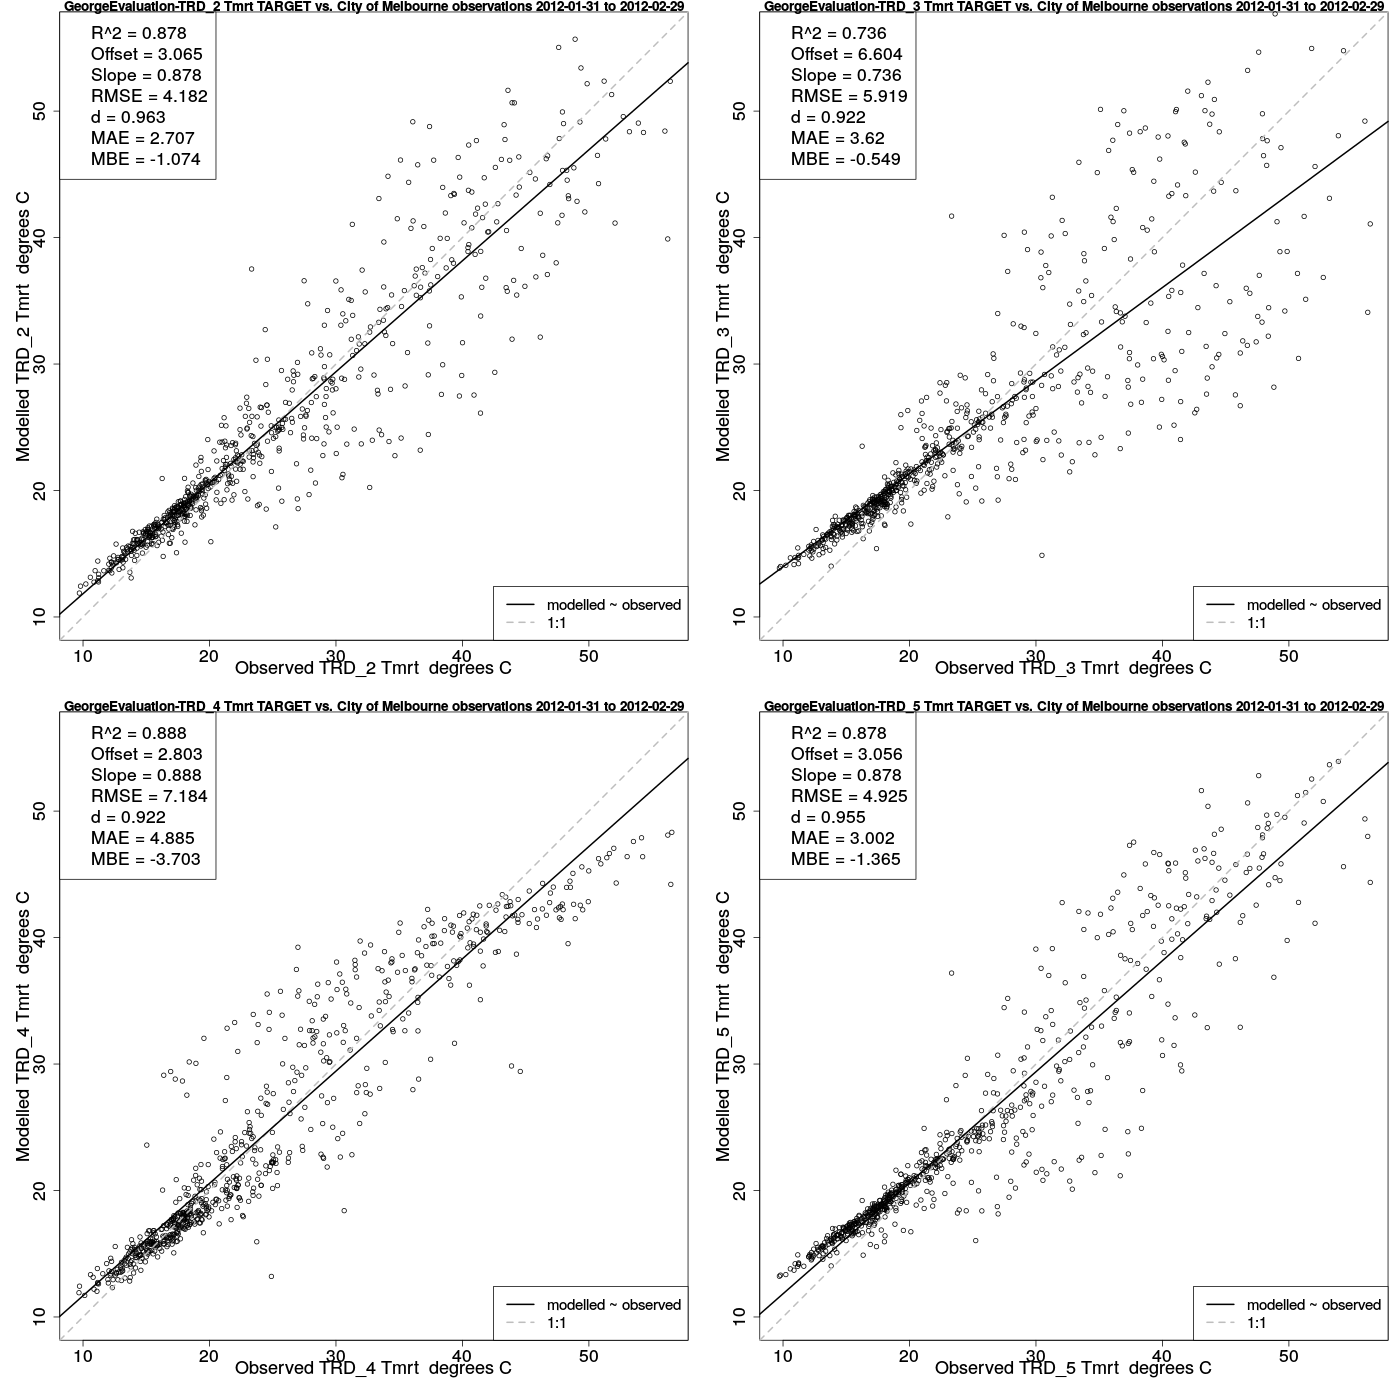
\includegraphics[scale=0.15]{images/Eval/GeorgeEvaluation-ErrorPlots-Tmrt.png}
~ b)
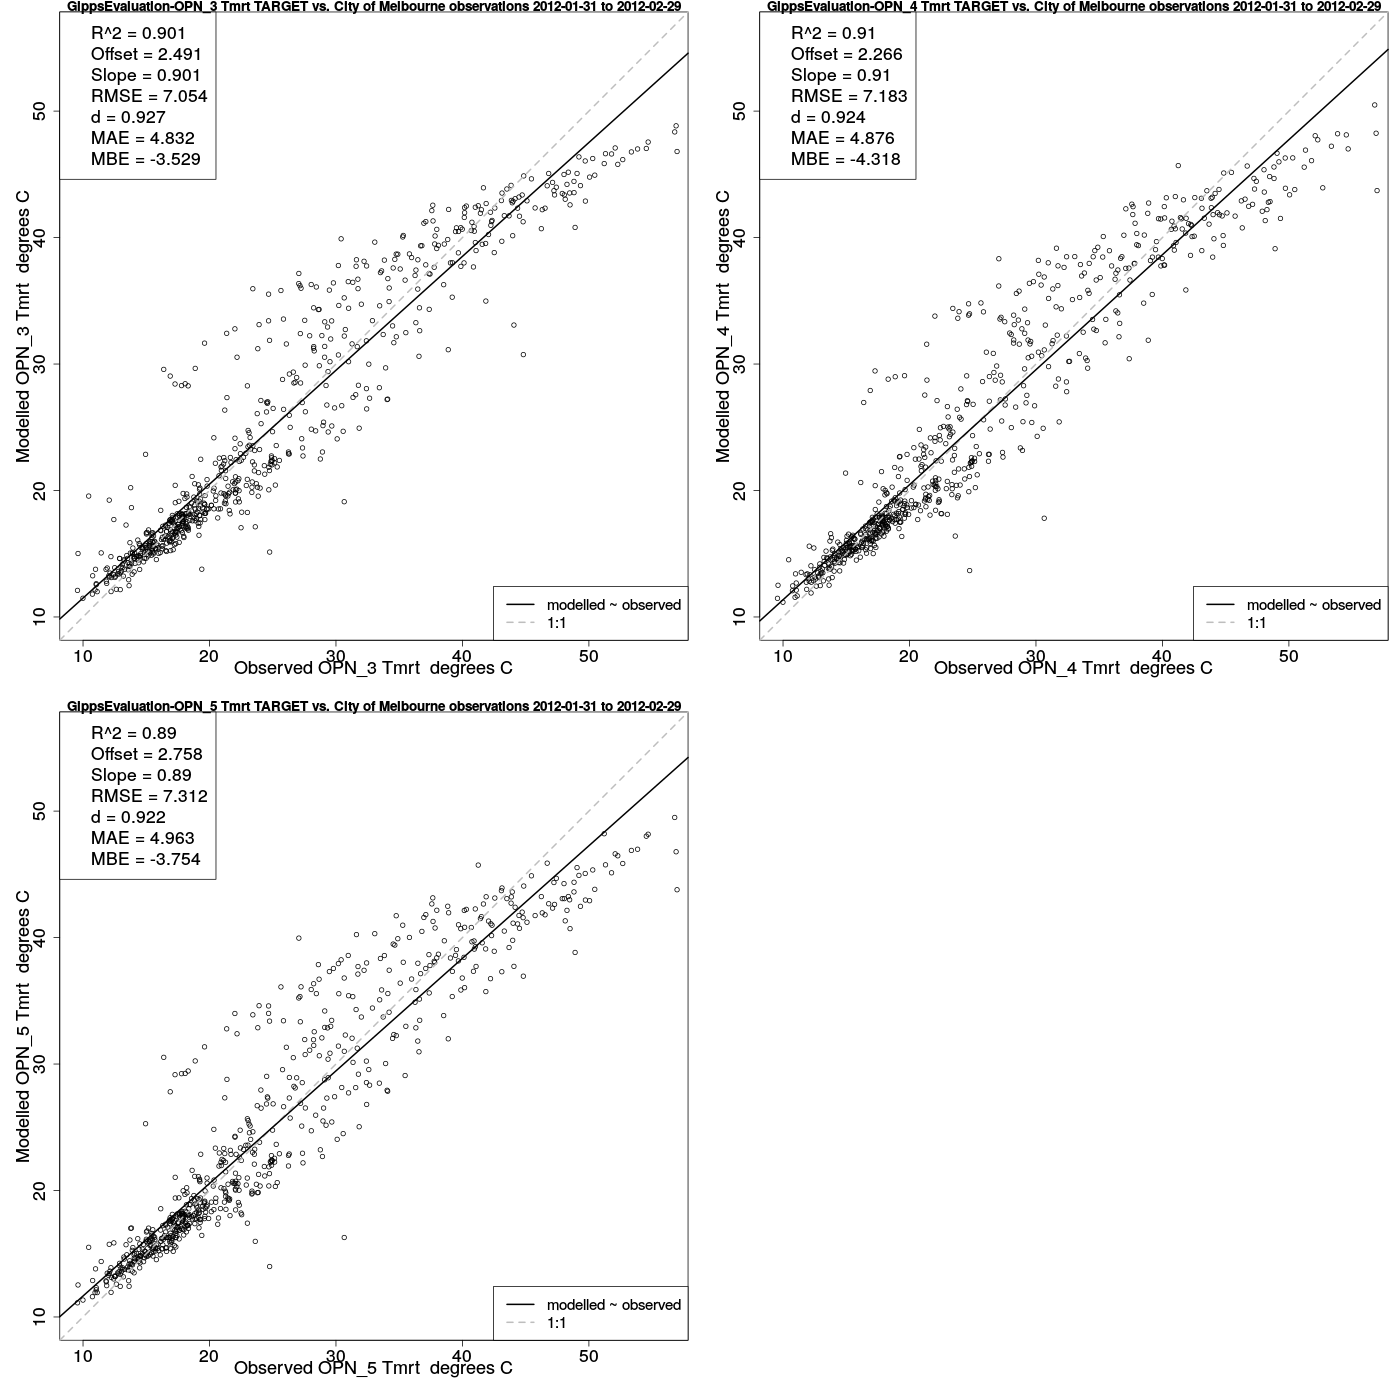
\includegraphics[scale=0.15]{images/Eval/GippsEvaluation-ErrorPlots-Tmrt.png}

\caption{\bf Comparison of TARGET modelled \glssymbol{Tmrt} to observed locations in a) George St. and b) Gipps St.}    
 \label{fig:tmrteval} 
\end{figure} 

\begin{figure}[!htbp]
a) 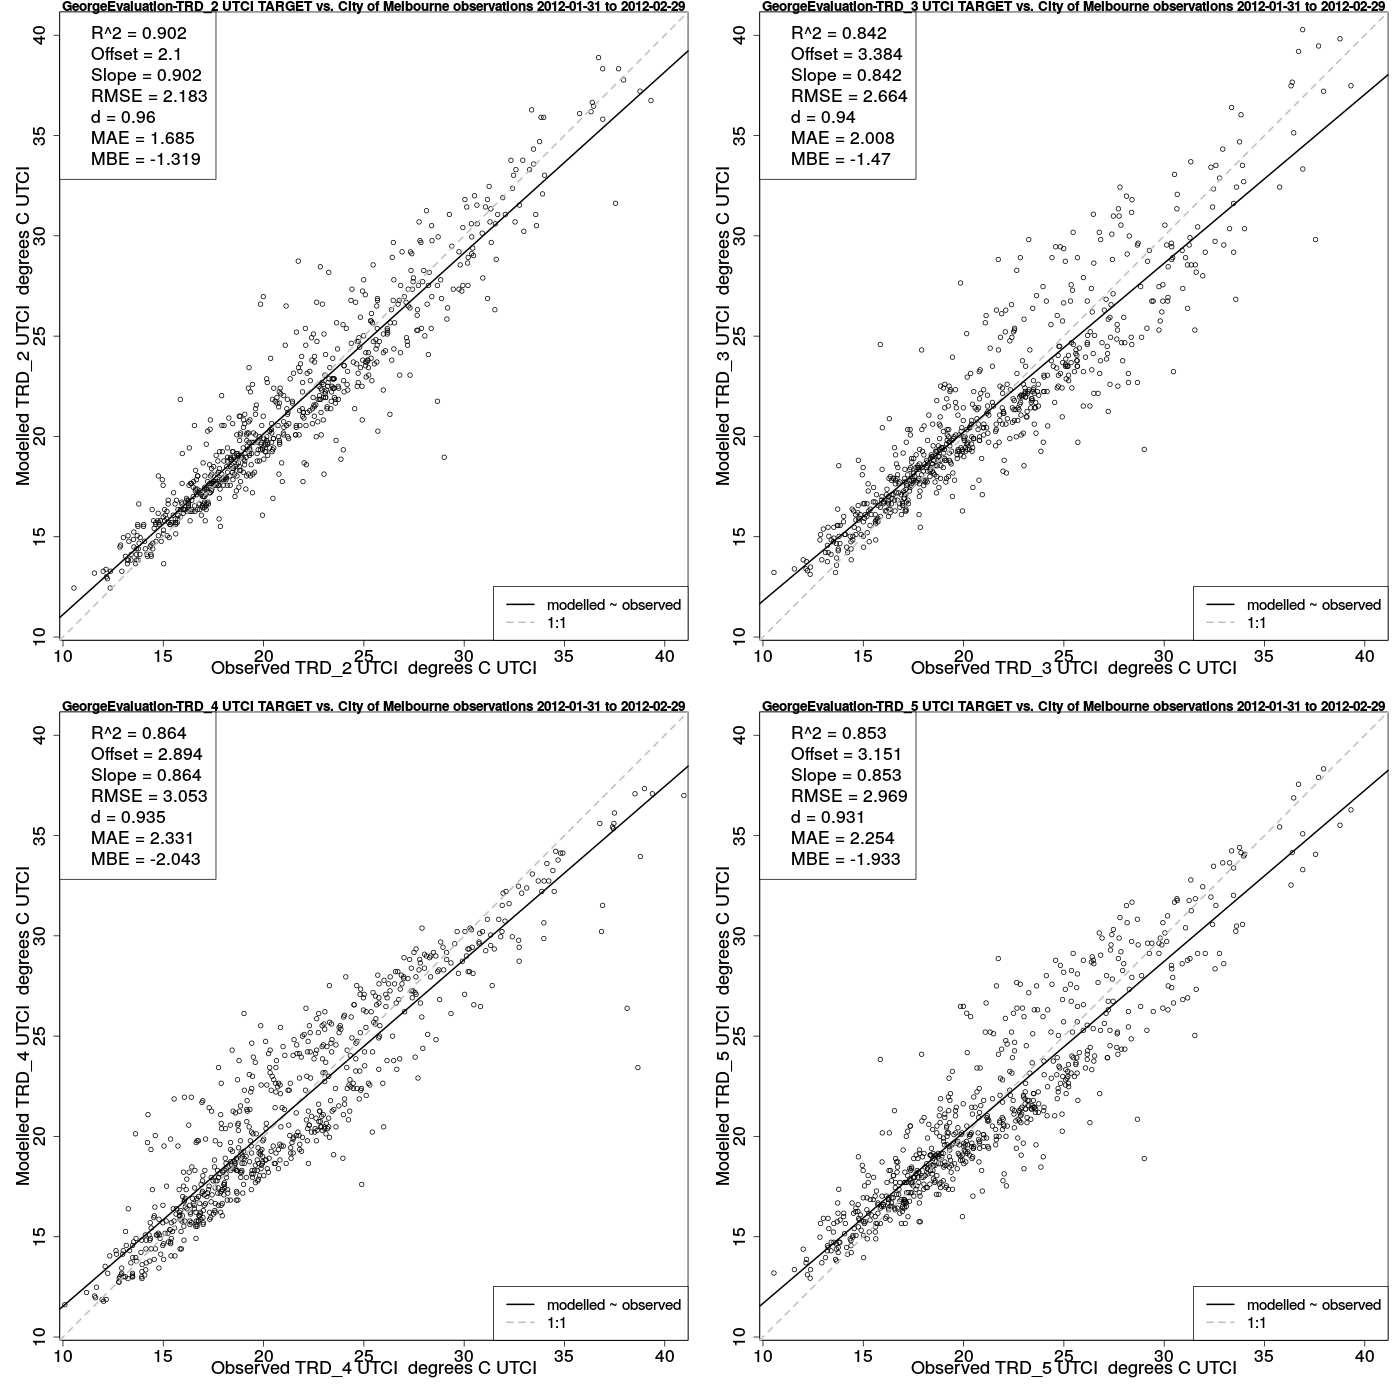
\includegraphics[scale=0.15]{images/Eval/GeorgeEvaluation-ErrorPlots-UTCI.png}
~ b)
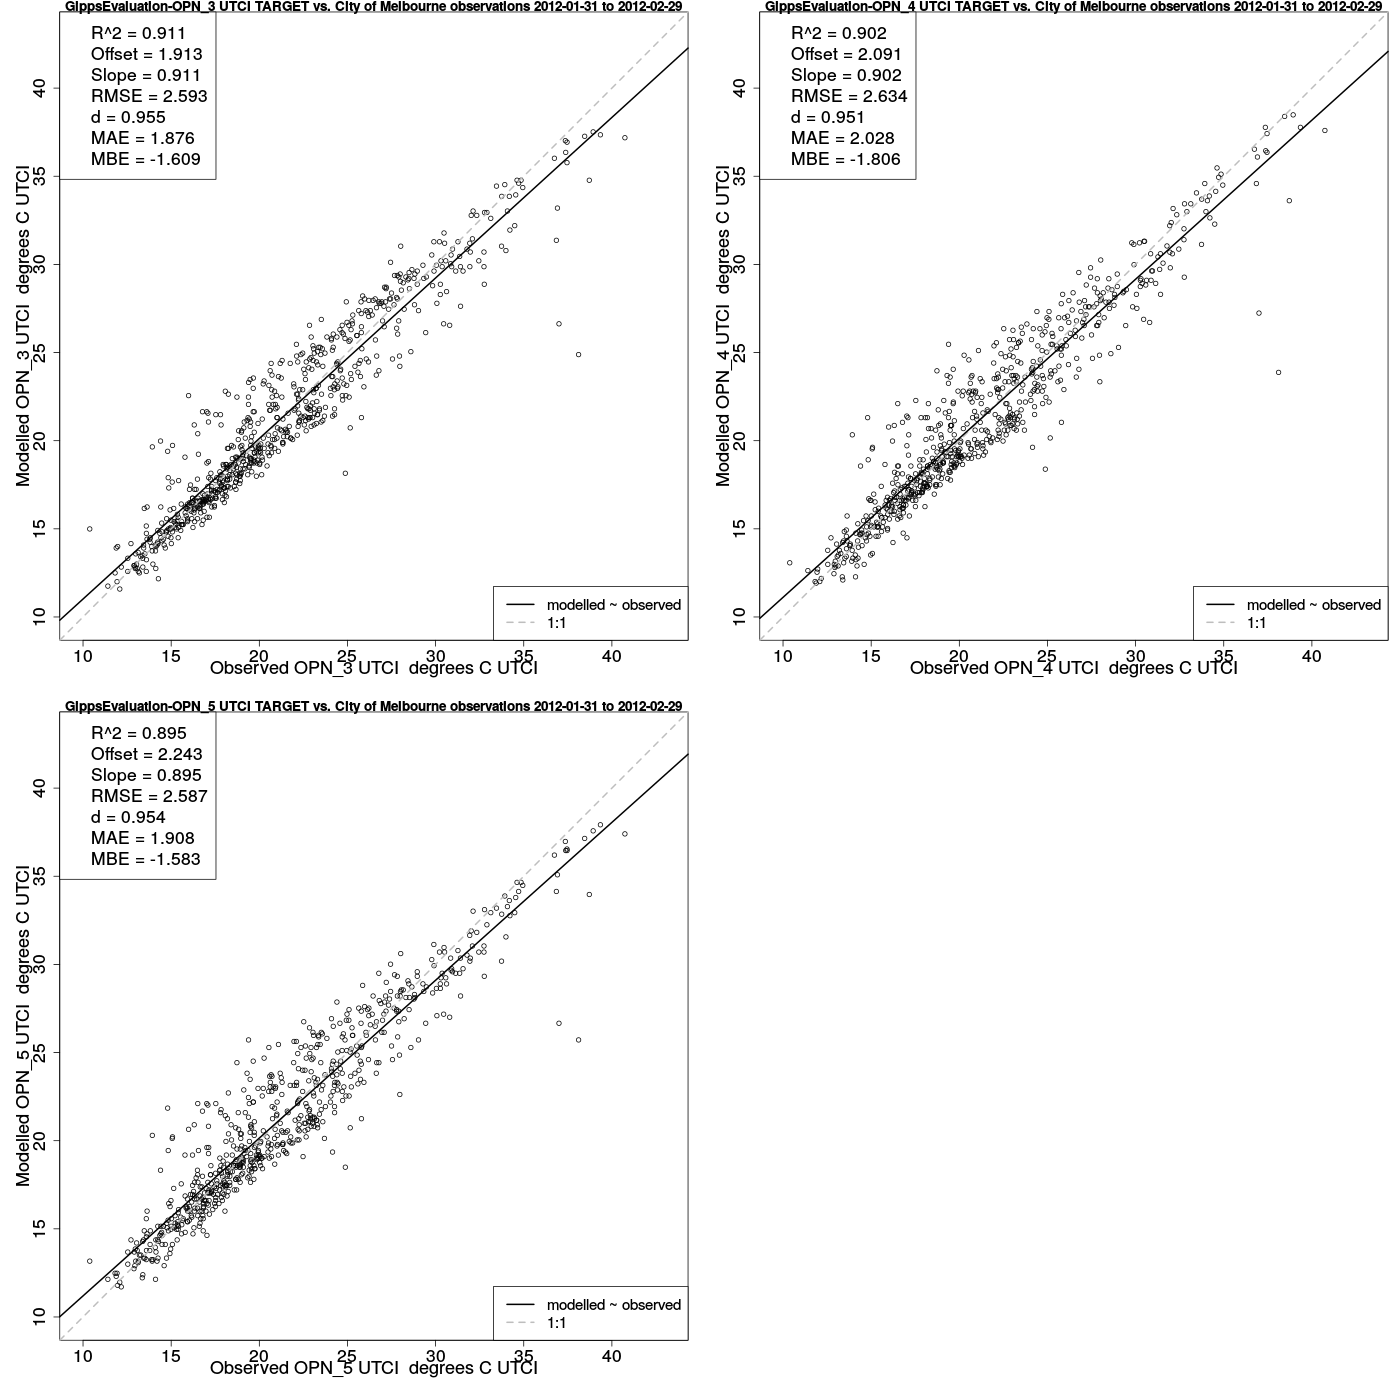
\includegraphics[scale=0.15]{images/Eval/GippsEvaluation-ErrorPlots-UTCI.png}

\caption{\bf Comparison of TARGET modelled \glssymbol{UTCI} to observed locations in a) George St. and b) Gipps St.}    
 \label{fig:utcieval} 
\end{figure} 


\begin{center}
\begin{table}
\caption{George St. GeorgeEvaluation and Gipps St. GippsEvaluation scenarios $T_{mrt}$ and UTCI predicted vs. observations statistical performance of RMSE (\SI{}{\degreeCelsius}), MBE (\SI{}{\degreeCelsius}), MAE (\SI{}{\degreeCelsius}), and d index of agreement.\label{tab:georgetmrt}}
  \begin{tabular}{ |c|c | c |c |c  | c | c |  c|c|}   
  \hline    &  \multicolumn{4}{c|}{\textbf{$T_{mrt}$}} & \multicolumn{4}{c|}{\textbf{UTCI}}  \\  
  \textbf{Observation point} 
	& \textbf{RMSE} 
	& \textbf{MBE} 
	& \textbf{MAE} 
	& \textbf{d} 
	& \textbf{RMSE} 
	& \textbf{MBE} 
	& \textbf{MAE}
	& \textbf{d}	
	\\ \hline
TRD\_2 & 4.18 & -1.07 & 2.71 & 0.963 & 2.18 & -1.32 & 1.69 & 0.960  \\ \hline
TRD\_3 & 5.92 & -0.55 & 3.62 & 0.922 & 2.66 & -1.47 & 2.01 & 0.940  \\ \hline
TRD\_4 & 7.18 & -3.70 & 4.89 & 0.922 & 3.05 & -2.04 & 2.33 & 0.935  \\ \hline
TRD\_5 & 4.93 & -1.37 & 3.00 & 0.955 & 2.97 & -1.93 & 2.25 & 0.931  \\ \hline
OPN\_3 & 7.05 & -3.53 & 4.83 & 0.927 & 2.59 & -1.61 & 1.88 & 0.955   \\ \hline
OPN\_4 & 7.18 & -4.32 & 4.88 & 0.924 & 2.63 & -1.81 & 2.03 & 0.951  \\ \hline
OPN\_5 & 7.31 & -3.75 & 4.96 & 0.922 & 2.59 & -1.59 & 1.90 & 0.954  \\ \hline
  \end{tabular} 
\end{table}
\end{center} 

Statistics for Gipps St., a street with an open canopy, show very similar results for each location, with d index of agreement values ranging from 0.922 to 0.927 for \glssymbol{Tmrt} and 0.951 to 0.955 for \glssymbol{UTCI}. George St. shows a slightly wider range of results with d index of agreement values ranging from 0.922 to 0.963 for \glssymbol{Tmrt} and 0.931 to 0.960 for \glssymbol{UTCI}. Slightly more accurate results for \glssymbol{Tmrt} for locations with morning shade and afternoon sun (TRD\_2 and TRD\_5) compared to the other locations with full sun. The most accurate predictions of \glssymbol{UTCI} were for TRD\_2, a location with more shading than the other TRD locations. 

Overall, the results show that the new HTC module in TARGET performs well is suitable to make HTC predictions for a variety of urban scenarios.

\subsection{Results of whole domain WSUD scenarios}\label{sec:whole_domain}
After the new functionality in the TARGET model has been evaluated to ensure accurate predictions, we turn to the results of the WSUD scenarios. 

The results of each of the scenarios were averaged across the entire 80,000 grid point domain for the 3 day modelling period. The difference in air temperature between WSUD Scenarios 1,3,4 and the control case Scenario 2, are shown for each climate scenario in Table \ref{tab:scenarioDiff}. Scenario 3 produced the most cooling in each climate scenario compared to the base case of Scenario 2, followed by Scenario 4. This was unexpected and suggests that for the whole domain the highest WSUD Scenario does not produce as much cooling throughout the three simulated days. However, the cooling produced in these simulations is extremely small, and may not be physical. There was no difference in temperature between Scenarios 1 and 2. 

Figure \ref{fig:diff_air_temp} shows differences in air temperature between the 4 WSUD scenarios for each of the 3 climate scenarios. As these are only averaged across the 80,000 grid point domain and not across the 3 day modelling period, they show larger differences at different times of the day. Averages at 2pm on the third day of the modelling period are summarized in Table \ref{tab:scenarioDiff}. These still show modest temperature reductions (around 0.1 to 0.2\SI{}{\degreeCelsius}) but of an order of magnitude larger than those averaged across the entire modelling period. Some slight warming at night of Scenario 4 would have offset some of the daytime temperature reductions in the 3 day average.

\begin{table}[!htbp]
\caption{\bf The difference in air temperature (average of the 80,000 grid points) across the 3 day modelling period and at 2pm on third day of the modelling period between WSUD scenarios for each climate scenario.  \label{tab:scenarioDiff}}     
\begin{tabular}{ l l l l l l l}
 \hline  \multicolumn{1}{|c}{}   &  \multicolumn{3}{|c|}{\textbf{3 day average}} & \multicolumn{3}{c|}{\textbf{2pm of third day average}}  \\
\textbf{Scenario difference} 
& \textbf{Cool (\SI{}{\degreeCelsius})}
& \textbf{Average (\SI{}{\degreeCelsius})}
& \textbf{Extreme (\SI{}{\degreeCelsius})}
& \textbf{Cool (\SI{}{\degreeCelsius})}
& \textbf{Average (\SI{}{\degreeCelsius})}
& \textbf{Extreme (\SI{}{\degreeCelsius})}
\\ \hline
Scenario 1 minus Scenario 2 & 0.0  & 0.0 & 0.0       &0.017&0.016&0.045\\ 
Scenario 3 minus Scenario 2 & -0.04  & -0.03 & -0.03 &-0.082&-0.077&-0.129\\ 
Scenario 4 minus Scenario 2 & -0.02  & -0.01 & -0.02 &-0.079&-0.074&-0.226\\ 
\hline
\end{tabular}
\end{table}

						
								



\begin{figure}[!htbp]
\centering   
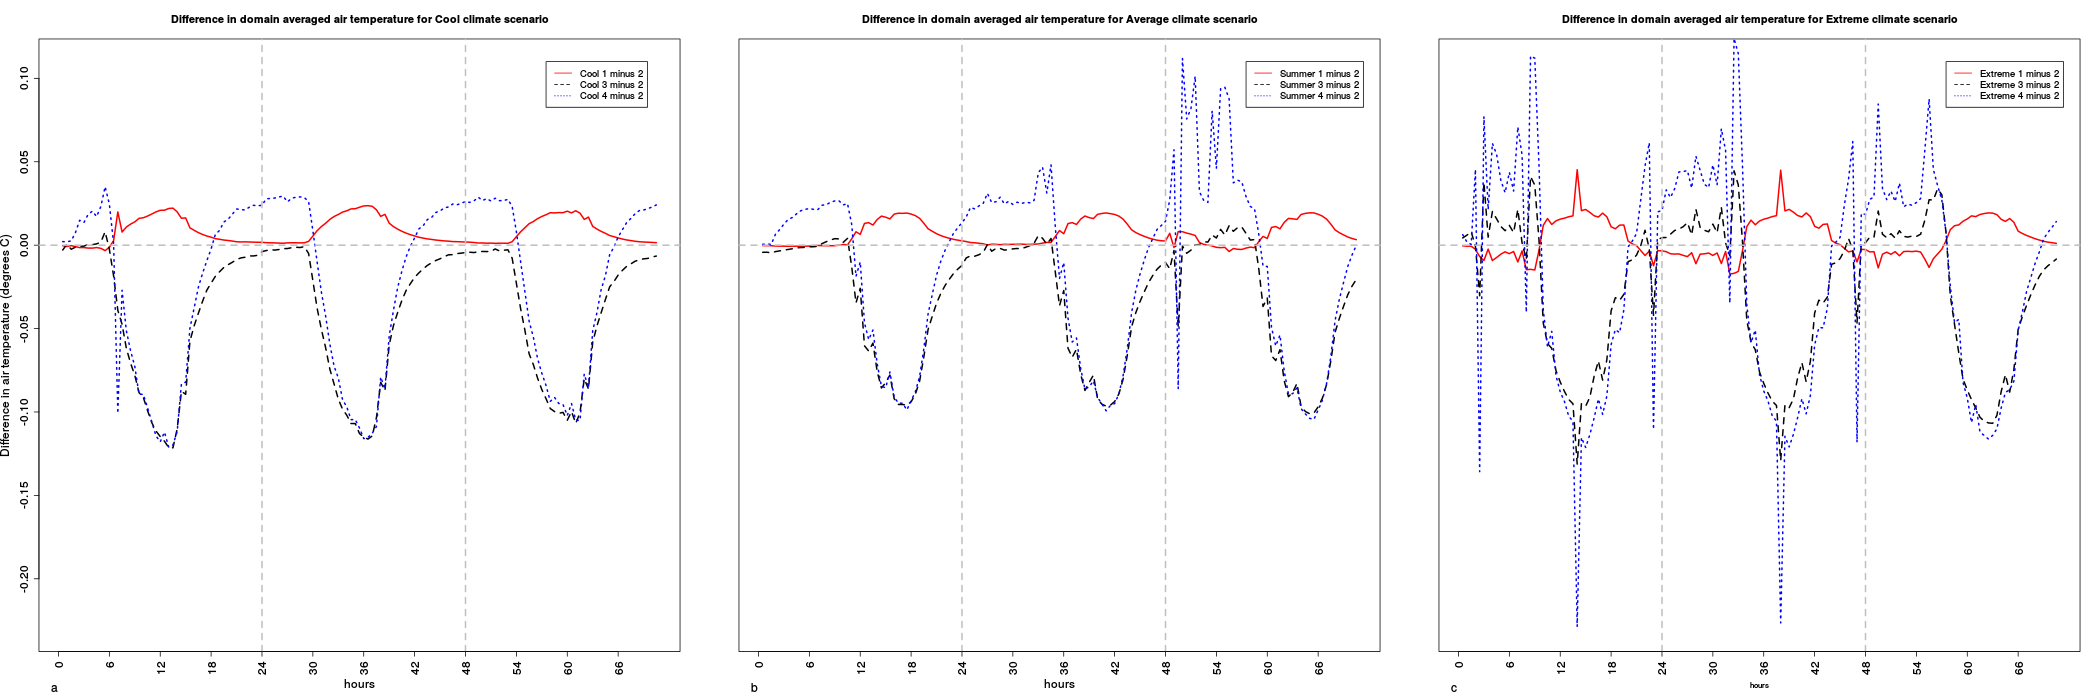
\includegraphics[scale=0.25]{images/temperatures/SunburyAll}
\caption{\bf Differences in air temperatures (\SI{}{\degreeCelsius}) (averaged across 80,000 domain grid points) for a) Cool, b) Average, and c) Extreme climate scenarios over the 3 day modelling period. }    
 \label{fig:diff_air_temp} 
\end{figure} 


Overall, the WSUD implemented in Scenario 3 can reduce the 2m air temperature by 0.04\SI{}{\degreeCelsius} during cool summer days, 0.03\SI{}{\degreeCelsius} during average summer days and 0.03\SI{}{\degreeCelsius} during extreme summer days, with larger temperature reductions of 0.1 to 0.2\SI{}{\degreeCelsius} during the hottest part of the day.


TODO the next paragraph isn't quite right with the 2pm averages. The Extreme days cool the most.

The noteworthy result is that WSUD is most effective during a cool summer day. To investigate this result, simulations where the whole domain consists of one land surface category were performed for each climate scenario. This was to understand how each land surface type responded to the cool, average and extreme summer days.

In these scenarios (Figures \ref{fig:surface_air_temps}a and b), it can be seen that during the cool days there is a clear difference in air temperature between the warmest land surface categories: road, concrete, and dry grass. In contrast, during extreme days the differences are much smaller between the categories. We hypothesise that during extreme days every surface type is extremely hot regardless of whether it is irrigated grass or concrete, accounting for the smaller difference in temperature from the high WSUD scenario during extreme days.


\begin{figure}[!htbp]
\centering   
a)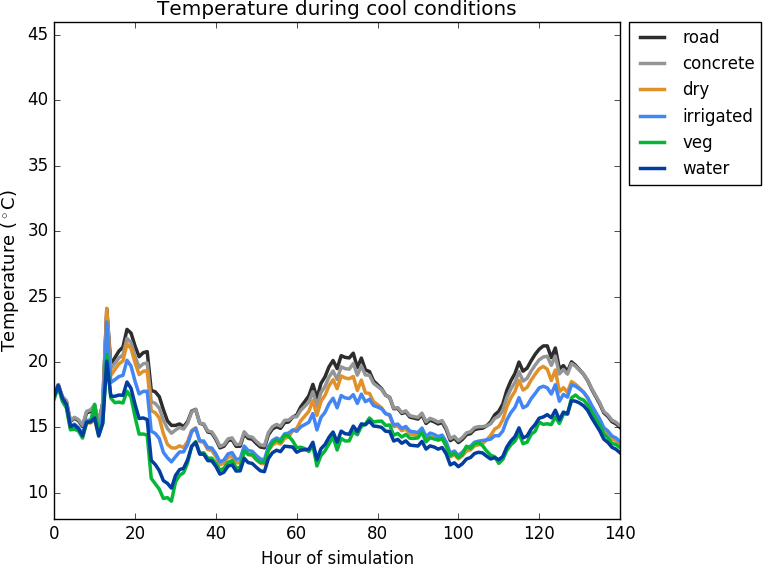
\includegraphics[scale=0.40]{images/fig1a}
~
b)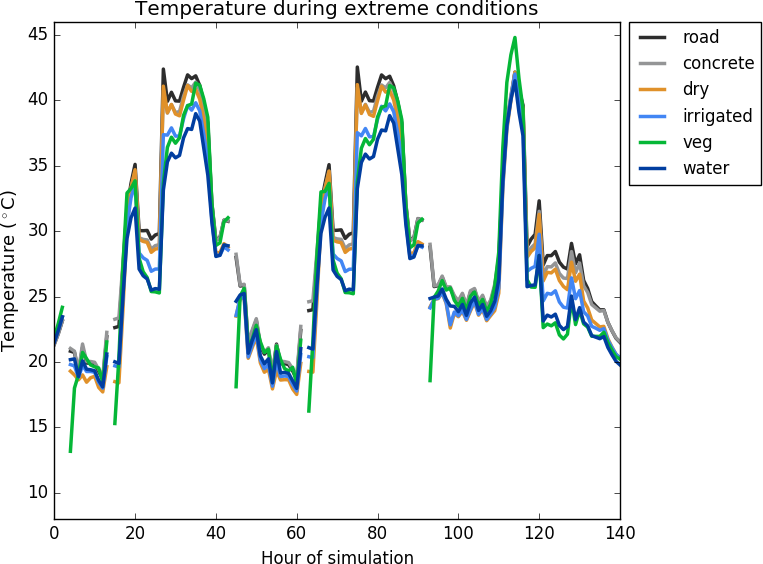
\includegraphics[scale=0.40]{images/fig1b} 
\caption{\bf The air temperature of each land surface category during a the three (a) cool and (b) extreme summer days. Missing points are from missing input data.}    
 \label{fig:surface_air_temps} 
\end{figure} 


\subsection{A small representative urban portion}\label{sec:result_rep_urban}
Averaging results over the whole domain is not necessarily representative of what would be experienced by a resident of the suburb, particularly since a large portion of the modelling domain is surrounding grasslands. Therefore, we conducted an analysis on a small representative urban portion (designated area of interest (AOI)), of the domain (highlighted in Figure \ref{fig:temp_diff_repre}), the results of which are discussed in this section. Also, all results discussed in Section \ref{sec:results_htc} are from the AOI.

\begin{figure}[!htbp]
\centering   
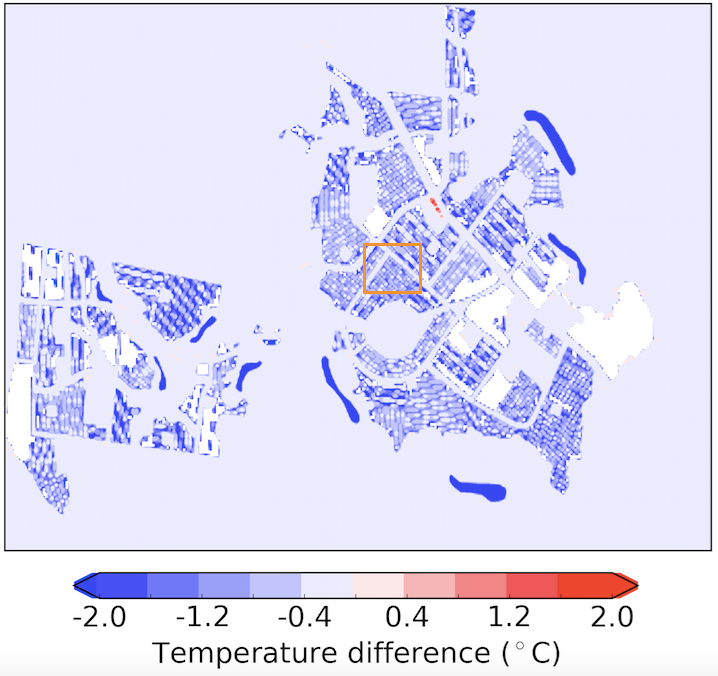
\includegraphics[scale=0.40]{images/fig2}
\caption{\bf The air temperature difference between Scenario 4 and Scenario 2 for the whole domain with the orange box indicating the small representative urban portion area of interest (AOI).}    
 \label{fig:temp_diff_repre} 
\end{figure}

The air temperature difference (averaged across the AOI during the three day scenario) between Scenarios 1, 3, and 4 and Scenario 2, the control case, are shown in Table \ref{tab:scenarioDiffRep}. These results are much more significant and align with expectations that Scenario 4 would produce the most cooling, followed by Scenario 3. The policy goal of Scenario 3 produces cooling of \textasciitilde 0.1\SI{}{\degreeCelsius} for each climate scenario. However, the efficacy of Scenario 4 is highly dependent on the climate scenario, producing an average cooling of 0.5\SI{}{\degreeCelsius} during the Cool Scenario, 0.4\SI{}{\degreeCelsius} during the Average Scenario and 0.3\SI{}{\degreeCelsius} during the Extreme Scenario. This follows the same logic from the previous section that the differences between each land surface category is larger during Cool summer days where WSUD can have a larger effect, but during Average and Extreme summer days all land surfaces (including vegetation and water) are warmer so it is harder for WSUD to create a cooling effect.


\begin{table}[!htbp]
\caption{\bf The difference in air temperature between the WSUD Scenarios for each Climate Scenario, averaged across the AOI during the three day scenario and at 2pm on the third day of the scenario. \label{tab:scenarioDiffRep}}     
\begin{tabular}{ l l l l l l l}
 \hline  \multicolumn{1}{|c}{}   &  \multicolumn{3}{|c|}{\textbf{3 day average}} & \multicolumn{3}{c|}{\textbf{2pm of third day average}}  \\
\textbf{Scenario difference} 
& \textbf{Cool (\SI{}{\degreeCelsius})}
& \textbf{Average (\SI{}{\degreeCelsius})}
& \textbf{Extreme (\SI{}{\degreeCelsius})}
& \textbf{Cool (\SI{}{\degreeCelsius})}
& \textbf{Average (\SI{}{\degreeCelsius})}
& \textbf{Extreme (\SI{}{\degreeCelsius})}
\\ \hline
Scenario 1 minus Scenario 2 & 0.0  & 0.0 & 0.0 &-0.012&-0.010&-0.004\\ 
Scenario 3 minus Scenario 2 & -0.12  & -0.10 & -0.10&-0.256&-0.239&-0.264\\ 
Scenario 4 minus Scenario 2 & -0.51  & -0.40 & -0.31&-0.888&-0.826&-0.688\\ 
\hline
\end{tabular}
\end{table}



The timeseries plots of the area average air temperature for each WSUD scenario (Figure \ref{fig:timeseries_scenarios}) further show that Scenario 4 is more effective during cool summer days than Extreme summer days. The difference in temperature between the four WSUD Scenarios increases when averaging over the AOI, compared to the whole domain in Section \ref{sec:whole_domain}. This is because the WSUD interventions are more concentrated across the AOI and so the effects are more significant. In the previous section the majority of the domain is dry grasslands which dilutes the cooling. The average difference in temperature between the WSUD scenarios is largest during the day (Figure \ref{fig:timeseries_scenarios}) indicating that the daily average reduction in temperature in Table \ref{tab:scenarioDiffRep} does not represent the diurnal effects of the cooling.

Another interesting finding is that WSUD is almost ineffectual at night (Figure \ref{fig:timeseries_scenarios}). This suggests that for reducing nighttime heat stress and improving human thermal comfort, these WSUD scenarios may not have the desired effect. Human thermal comfort outcomes will be discussed further in the next section.

\begin{figure}[!htbp]
\centering   
a)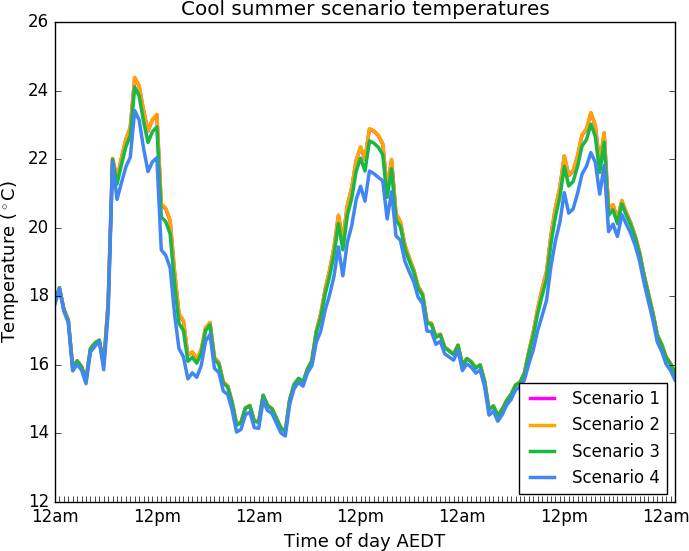
\includegraphics[scale=0.40]{images/fig3a}
~
b)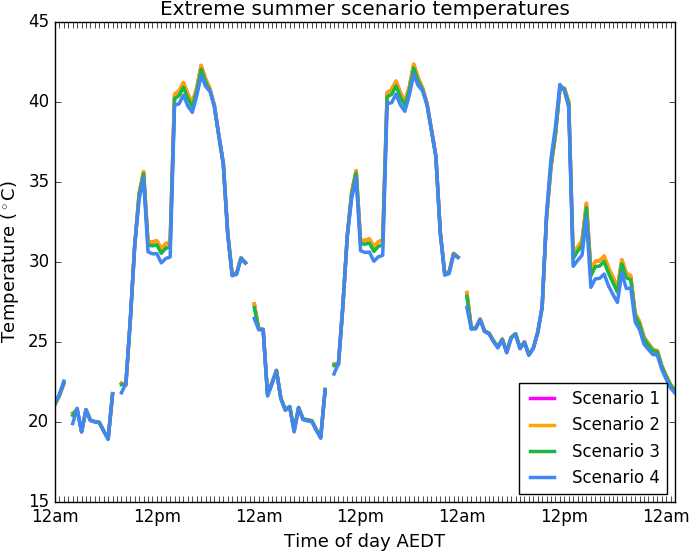
\includegraphics[scale=0.40]{images/fig3b} 
\caption{\bf The timeseries of air temperatures for the four WSUD Scenarios during the (a) Cool Scenario and (b) Extreme Scenario. Gaps are from missing data.}    
 \label{fig:timeseries_scenarios} 
\end{figure} 




\subsection{Human thermal comfort impacts of WSUD}\label{sec:results_htc}

With the additions to the TARGET model described in Section \ref{sec:tmrtutci}, TARGET is now able to output the Universal Thermal Climate Index (\glssymbol{UTCI}), a measure of how a person feels that accounts for temperature, wind speed, relative humidity and radiation through the mean radiant temperature. Using the \glssymbol{UTCI} gives further detail into how WSUD changes the environment for humans. For example, the temperature may be reduced due to irrigated grass but people may not feel the difference due to the added humidity, which can make an environment feel warmer to a person.

The average difference in \glssymbol{UTCI} between WSUD Scenarios 1, 3, and 4 and Scenario 2 for the three climate scenarios are shown in Table \ref{tab:scenarioDiffRep2}. The reduction in \glssymbol{UTCI} (Table \ref{tab:scenarioDiffRep2}) is greater than the reduction in temperature in Table \ref{tab:scenarioDiffRep}. These results indicate that incorporating WSUD into the landscape (Scenario 4) is highly beneficial for increasing the cooling effect `felt' by humans. In terms of temperature, Scenario 4 cools by 0.51\SI{}{\degreeCelsius} during a Cool summer day, but the \glssymbol{UTCI} shows that it ‘feels’ like cooling of 0.81\SI{}{\degreeCelsius}, meaning that WSUD is effective at cooling the environment and improving human thermal comfort. Scenario 3 (which incorporates less WSUD interventions than Scenario 4) also produces significant cooling in the \glssymbol{UTCI} with reductions of 0.22\SI{}{\degreeCelsius} during Cool summer days. As with the temperature, the efficacy of the cooling of the \glssymbol{UTCI} is dependent on the climate scenario where the Cool Scenario has the most cooling and the Extreme Scenario has the least cooling. 

The difference in \glssymbol{UTCI} between Scenarios 1 and 2 show that Scenario 1 (the no WSUD Scenario) is cooler than the control case of Scenario 2. This is a counter intuitive result as Scenario 1 would be expected to be warmer than Scenario 2. However, the differences between the land surfaces are very small (Table 1) where Scenario 2 is almost identical except more water. As such, the difference in \glssymbol{UTCI} between the two scenarios is not considered physical. 


\begin{table}[!htbp]
\caption{\bf The difference in \glssymbol{UTCI} temperature between the WSUD Scenarios for each climate scenario for the AOI averaged across the three day scenario and at 2pm on the third day. \label{tab:scenarioDiffRep2}}     
\begin{tabular}{ l l l l l l l}
 \hline  \multicolumn{1}{|c}{}   &  \multicolumn{3}{|c|}{\textbf{3 day average}} & \multicolumn{3}{c|}{\textbf{2pm of third day average}}  \\
\textbf{Scenario difference} 
& \textbf{Cool (\SI{}{\degreeCelsius})}
& \textbf{Average (\SI{}{\degreeCelsius})}
& \textbf{Extreme (\SI{}{\degreeCelsius})}
& \textbf{Cool (\SI{}{\degreeCelsius})}
& \textbf{Average (\SI{}{\degreeCelsius})}
& \textbf{Extreme (\SI{}{\degreeCelsius})}
\\ \hline
Scenario 1 minus Scenario 2 & -0.02  & -0.01 & -0.02 &-0.015&-0.032&-0.004\\ 
Scenario 3 minus Scenario 2 & -0.22  & -0.19 & -0.14 &-0.627&-0.388&-0.381\\ 
Scenario 4 minus Scenario 2 & -0.81  & -0.68 & -0.38 &-2.123&-1.200&-1.009\\ 
\hline
\end{tabular}
\end{table}



Scenario 4 was designed to produce 2\SI{}{\degreeCelsius} of cooling and this is achieved when considering the spatial difference in \glssymbol{UTCI} compared to Scenario 2 at midday (Figure \ref{fig:fig4}). The 2\SI{}{\degreeCelsius} of cooling is almost everywhere during the Cool Scenarios and less pervasive in the Average and Extreme Scenarios, but these results are still significant. A reduction in \glssymbol{UTCI} of 2\SI{}{\degreeCelsius} has the potential to save many lives during summer (CITE).


\begin{figure}[!htbp]
\centering  
~~\textbf{{\small Cool Scenario 4 minus Scenario 2}} ~~~~
\textbf{{\small Average Scenario 4 minus Scenario 2}} ~~~~
\textbf{{\small Extreme Scenario 4 minus Scenario 2}} 
a)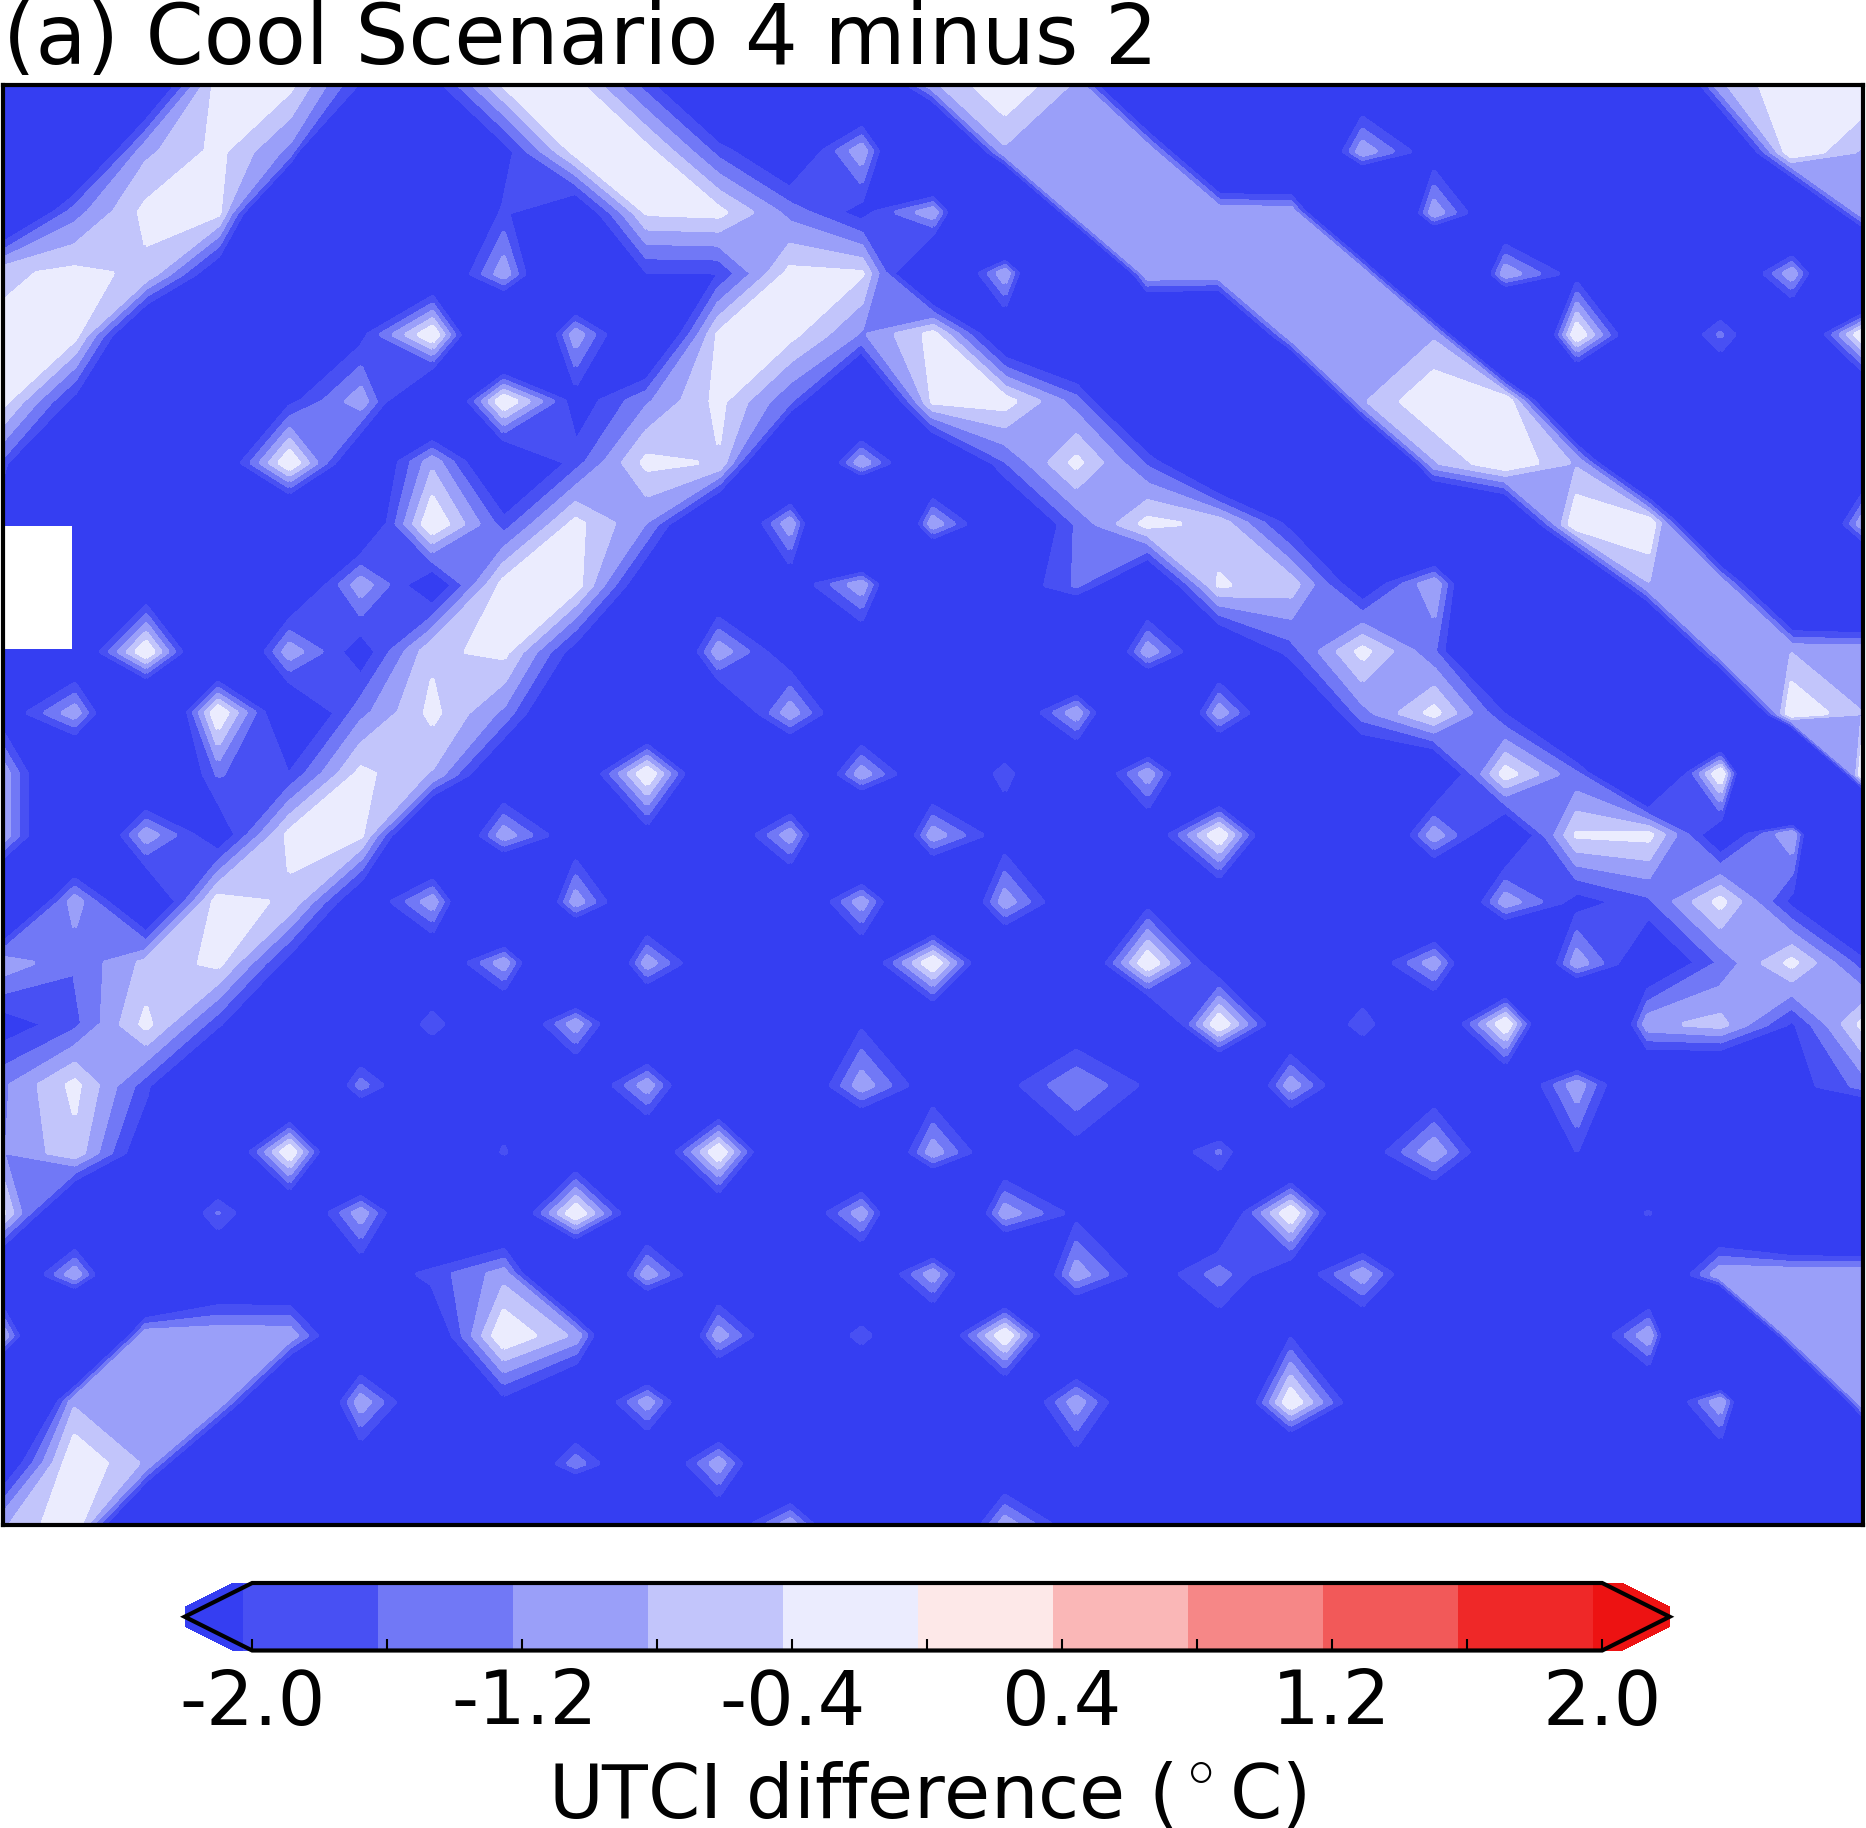
\includegraphics[scale=0.30,trim = 0mm 0mm 0mm 8mm,clip]{images/fig4a}
~
b)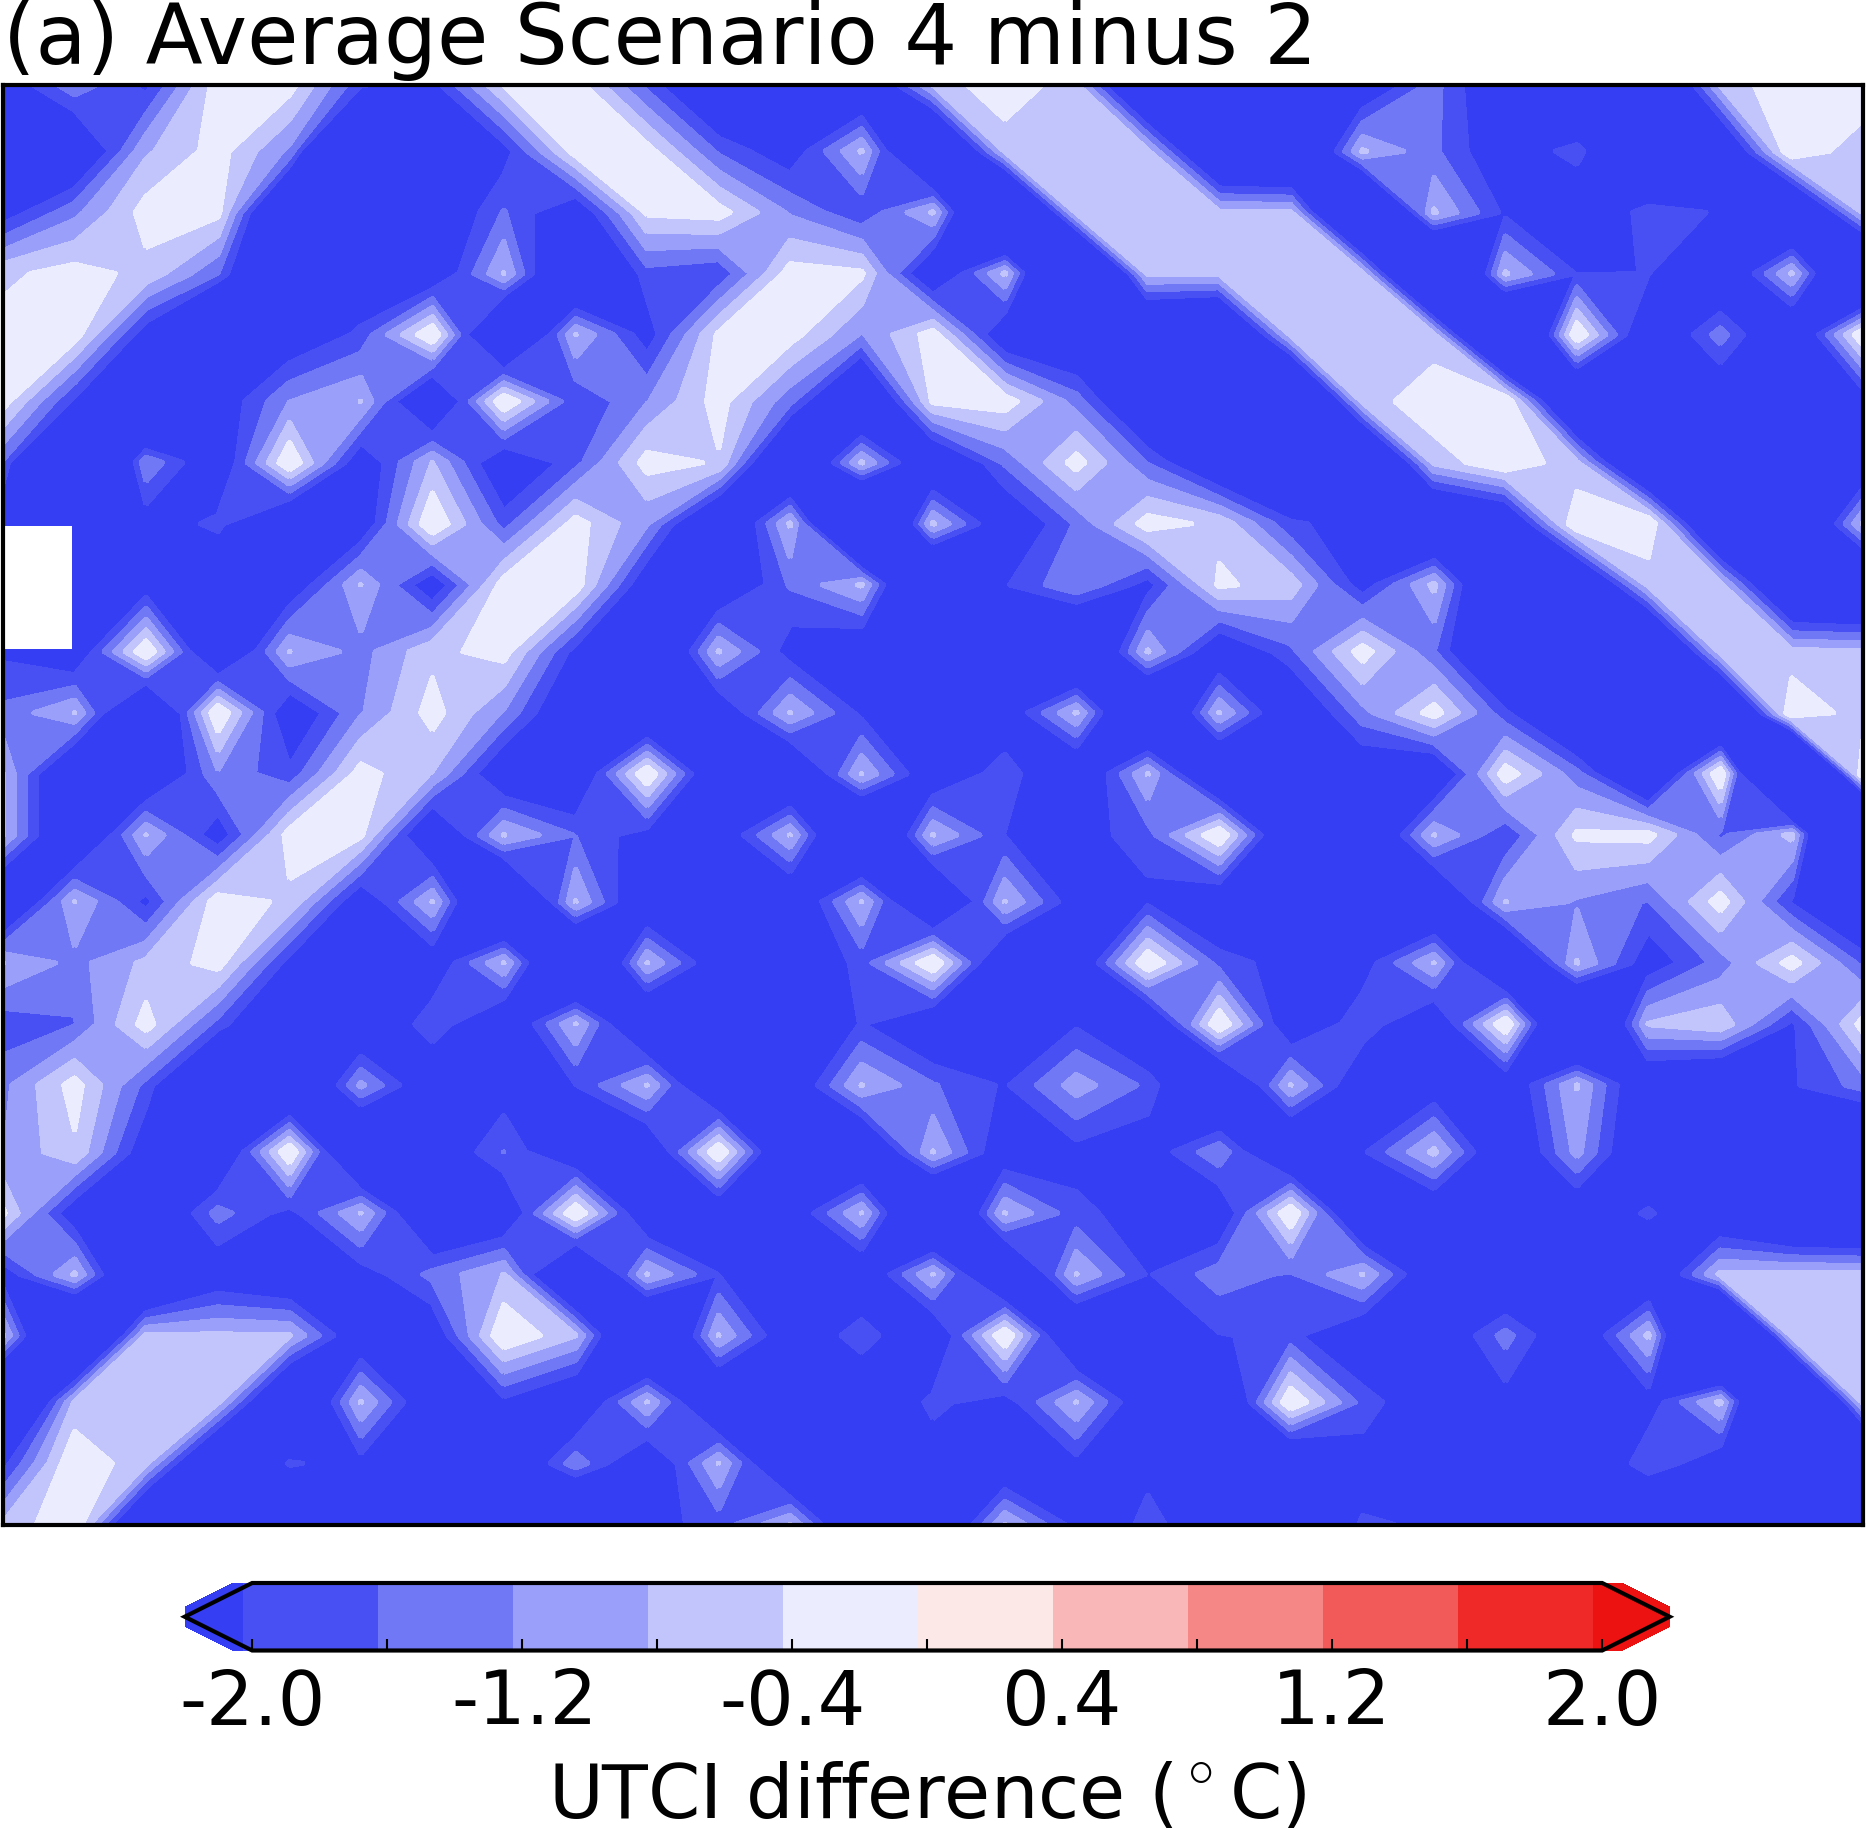
\includegraphics[scale=0.30,trim = 0mm 0mm 0mm 8mm,clip]{images/fig4b} 
~
c)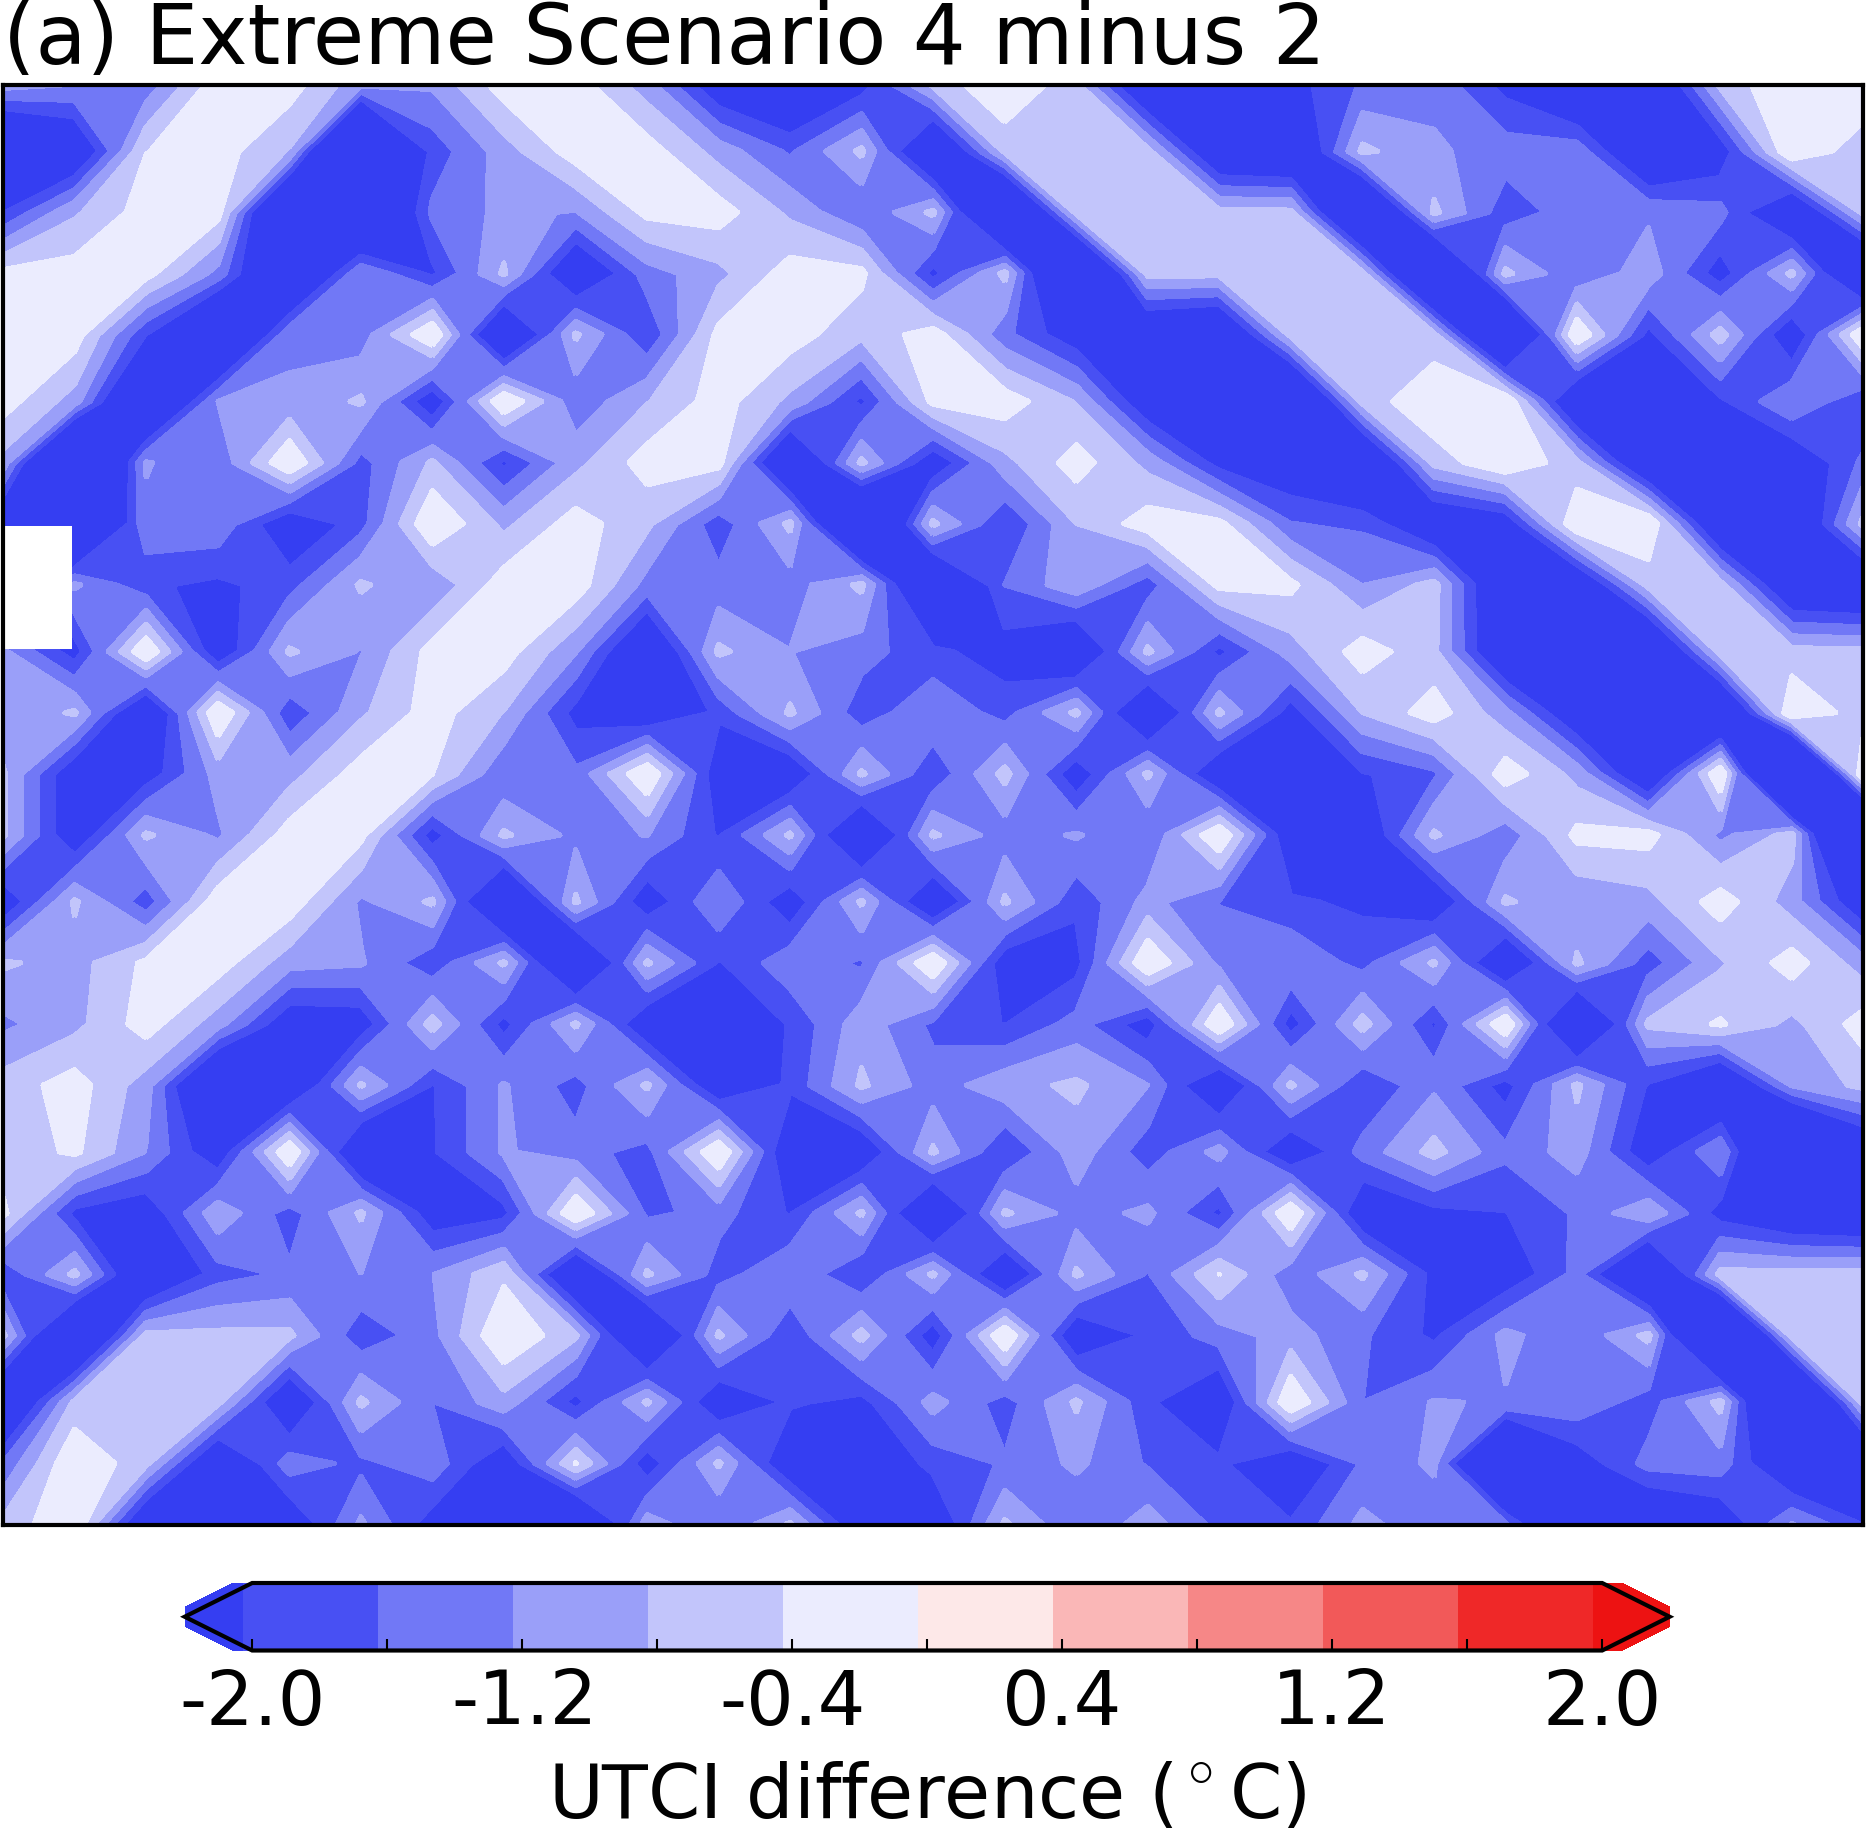
\includegraphics[scale=0.30,trim = 0mm 0mm 0mm 8mm,clip]{images/fig4c} 
\caption{\bf The difference in \glssymbol{UTCI} between Scenario 4 and Scenario 2 at midday for the AOI for the a) Cool, b) Average and c) Extreme climate Scenarios.}    
 \label{fig:fig4} 
\end{figure} 


%\subsection{Data for economic analysis}\label{sec:results_econ}
%To conduct the economic evaluation of the cooling from WSUD the maximum and minimum temperatures from a cool, average and extreme summer were reconstructed based on the modelling results from the four WSUD Scenarios and three Climate Scenarios. First, average summer temperatures (Dec - Feb) for Victoria were ranked from 1910-2017 and a typical cool summer (1986-87), an average summer (1971-1972) and an extreme summer (2008-2009) were identified. Maximum and minimum temperature data from Melbourne Airport weather station was then obtained for all 90 days (or 91 days for 1971-1972) of the three summers. The aim was to recreate the temperature during these summers if WSUD was present at the time, ie map the temperatures for the cases of Scenarios 1, 3 and 4, where Scenario 2 is observations. This was achieved by selecting the maximum and minimum temperature for each WSUD Scenario from the middle day of the Cool, Average and Extreme three day Scenarios described in Section \ref{sec:methods_wsudscenarios}. Using this data a linear interpolation was performed which creates an algorithm whereby data fed into the algorithm acts based on how much cooling each WSUD Scenario produced in each Climate Scenario. For example, data fed into the algorithm will have a larger reduction in temperature for cool days than extremely hot days, because the WSUD Scenarios are more effective during cool summer days than hot summer days. Hence, December 1 2008 had a maximum temperature of 21.1\SI{}{\degreeCelsius} but if WSUD Scenario 4 was implemented the algorithm says that the temperature would have been 19.7\SI{}{\degreeCelsius}, a difference of 1.4\SI{}{\degreeCelsius}. Furthermore, February 27 2009 had a temperature of 35.5\SI{}{\degreeCelsius} but if WSUD Scenario 4 was implemented the algorithm says that the temperature would have been 34.8\SI{}{\degreeCelsius}, a difference of 0.7\SI{}{\degreeCelsius}, showing that Scenario 4 is less effective on hotter days, as the modelling results showed.
%
%The maximum and minimum temperature from the typical cool (1986-87), average (1971-1972) and extreme summers (2008-2009) were put through the algorithm and the output was used to conduct the economic analysis. Figure \ref{fig:fig5}a is an example of this output for the 2008-2009 summer comparing the maximum temperatures of Scenario 2 (observations) and if there had of been a Scenario 4 level of WSUD present. The largest differences occur during the cooler days and the smallest differences occur on the hottest days. The two purple boxes indicate the January 28-30 2009 heatwave and the February 7 2009 Black Saturday event. Figure \ref{fig:fig5}b shows the same output for the minimum temperature where the differences between the scenarios is small.
%
%
%
%\begin{figure}[!htbp]
%\centering   
%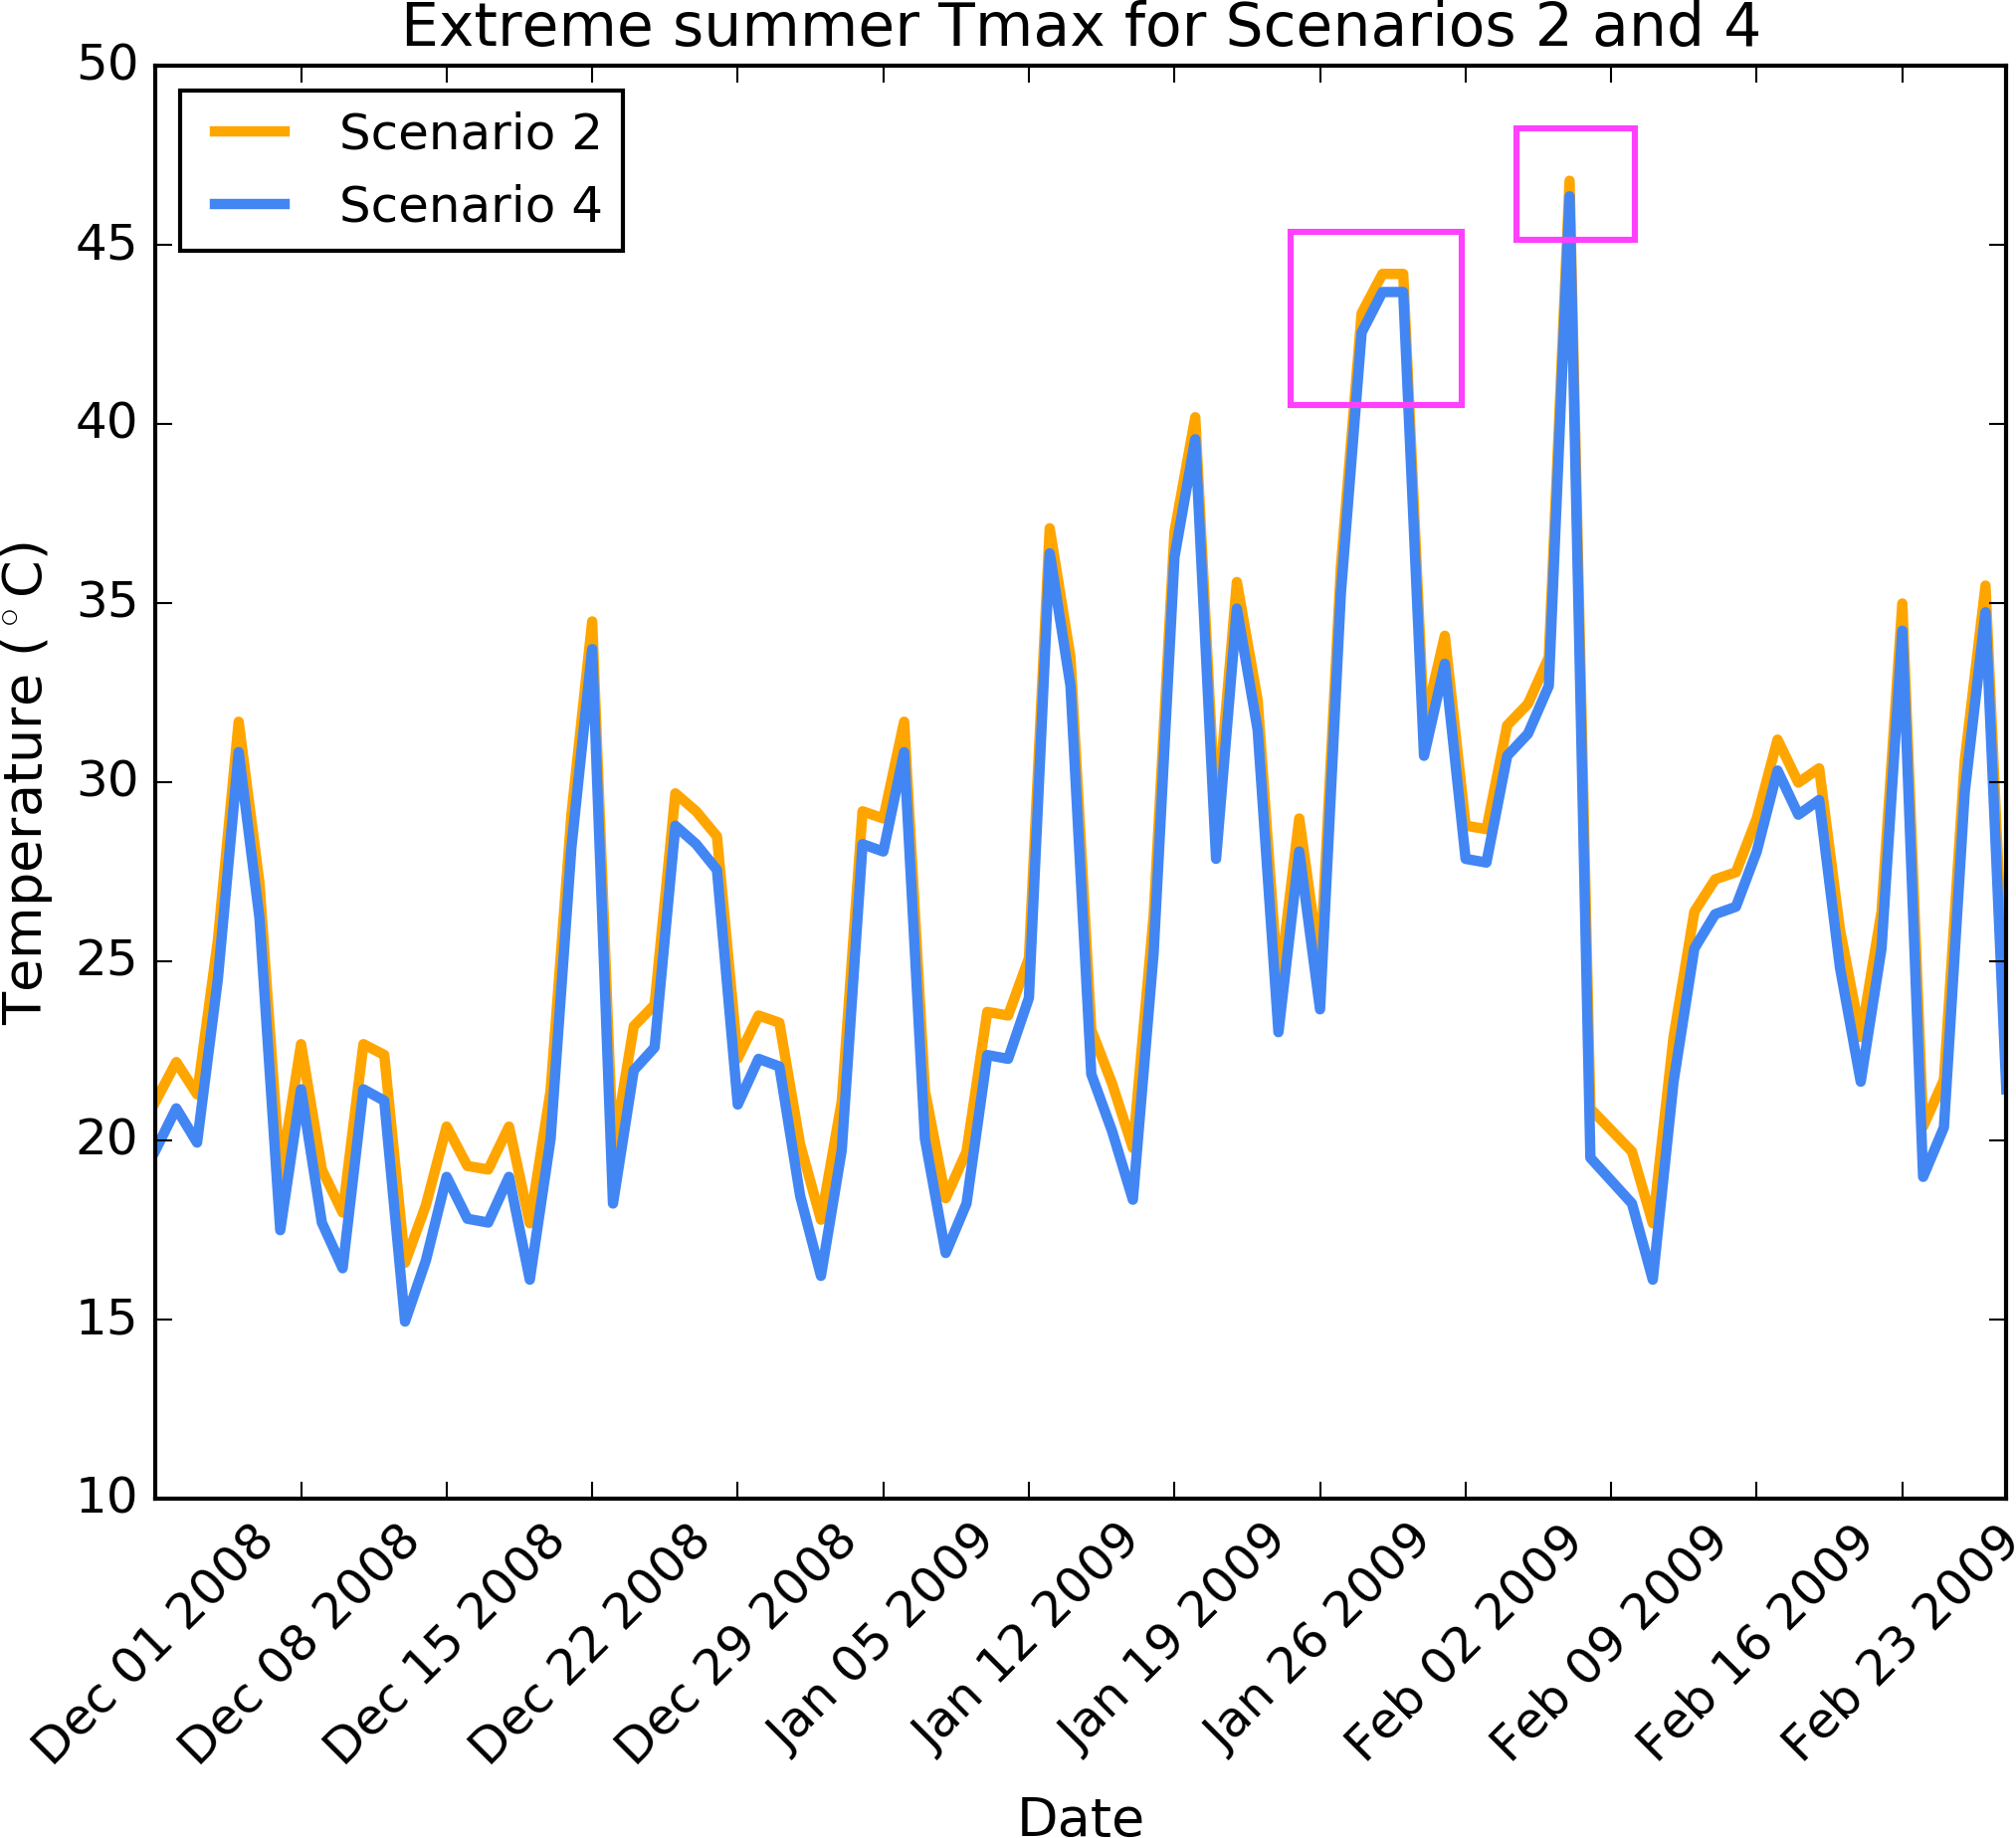
\includegraphics[scale=0.40]{images/fig5a}
%~
%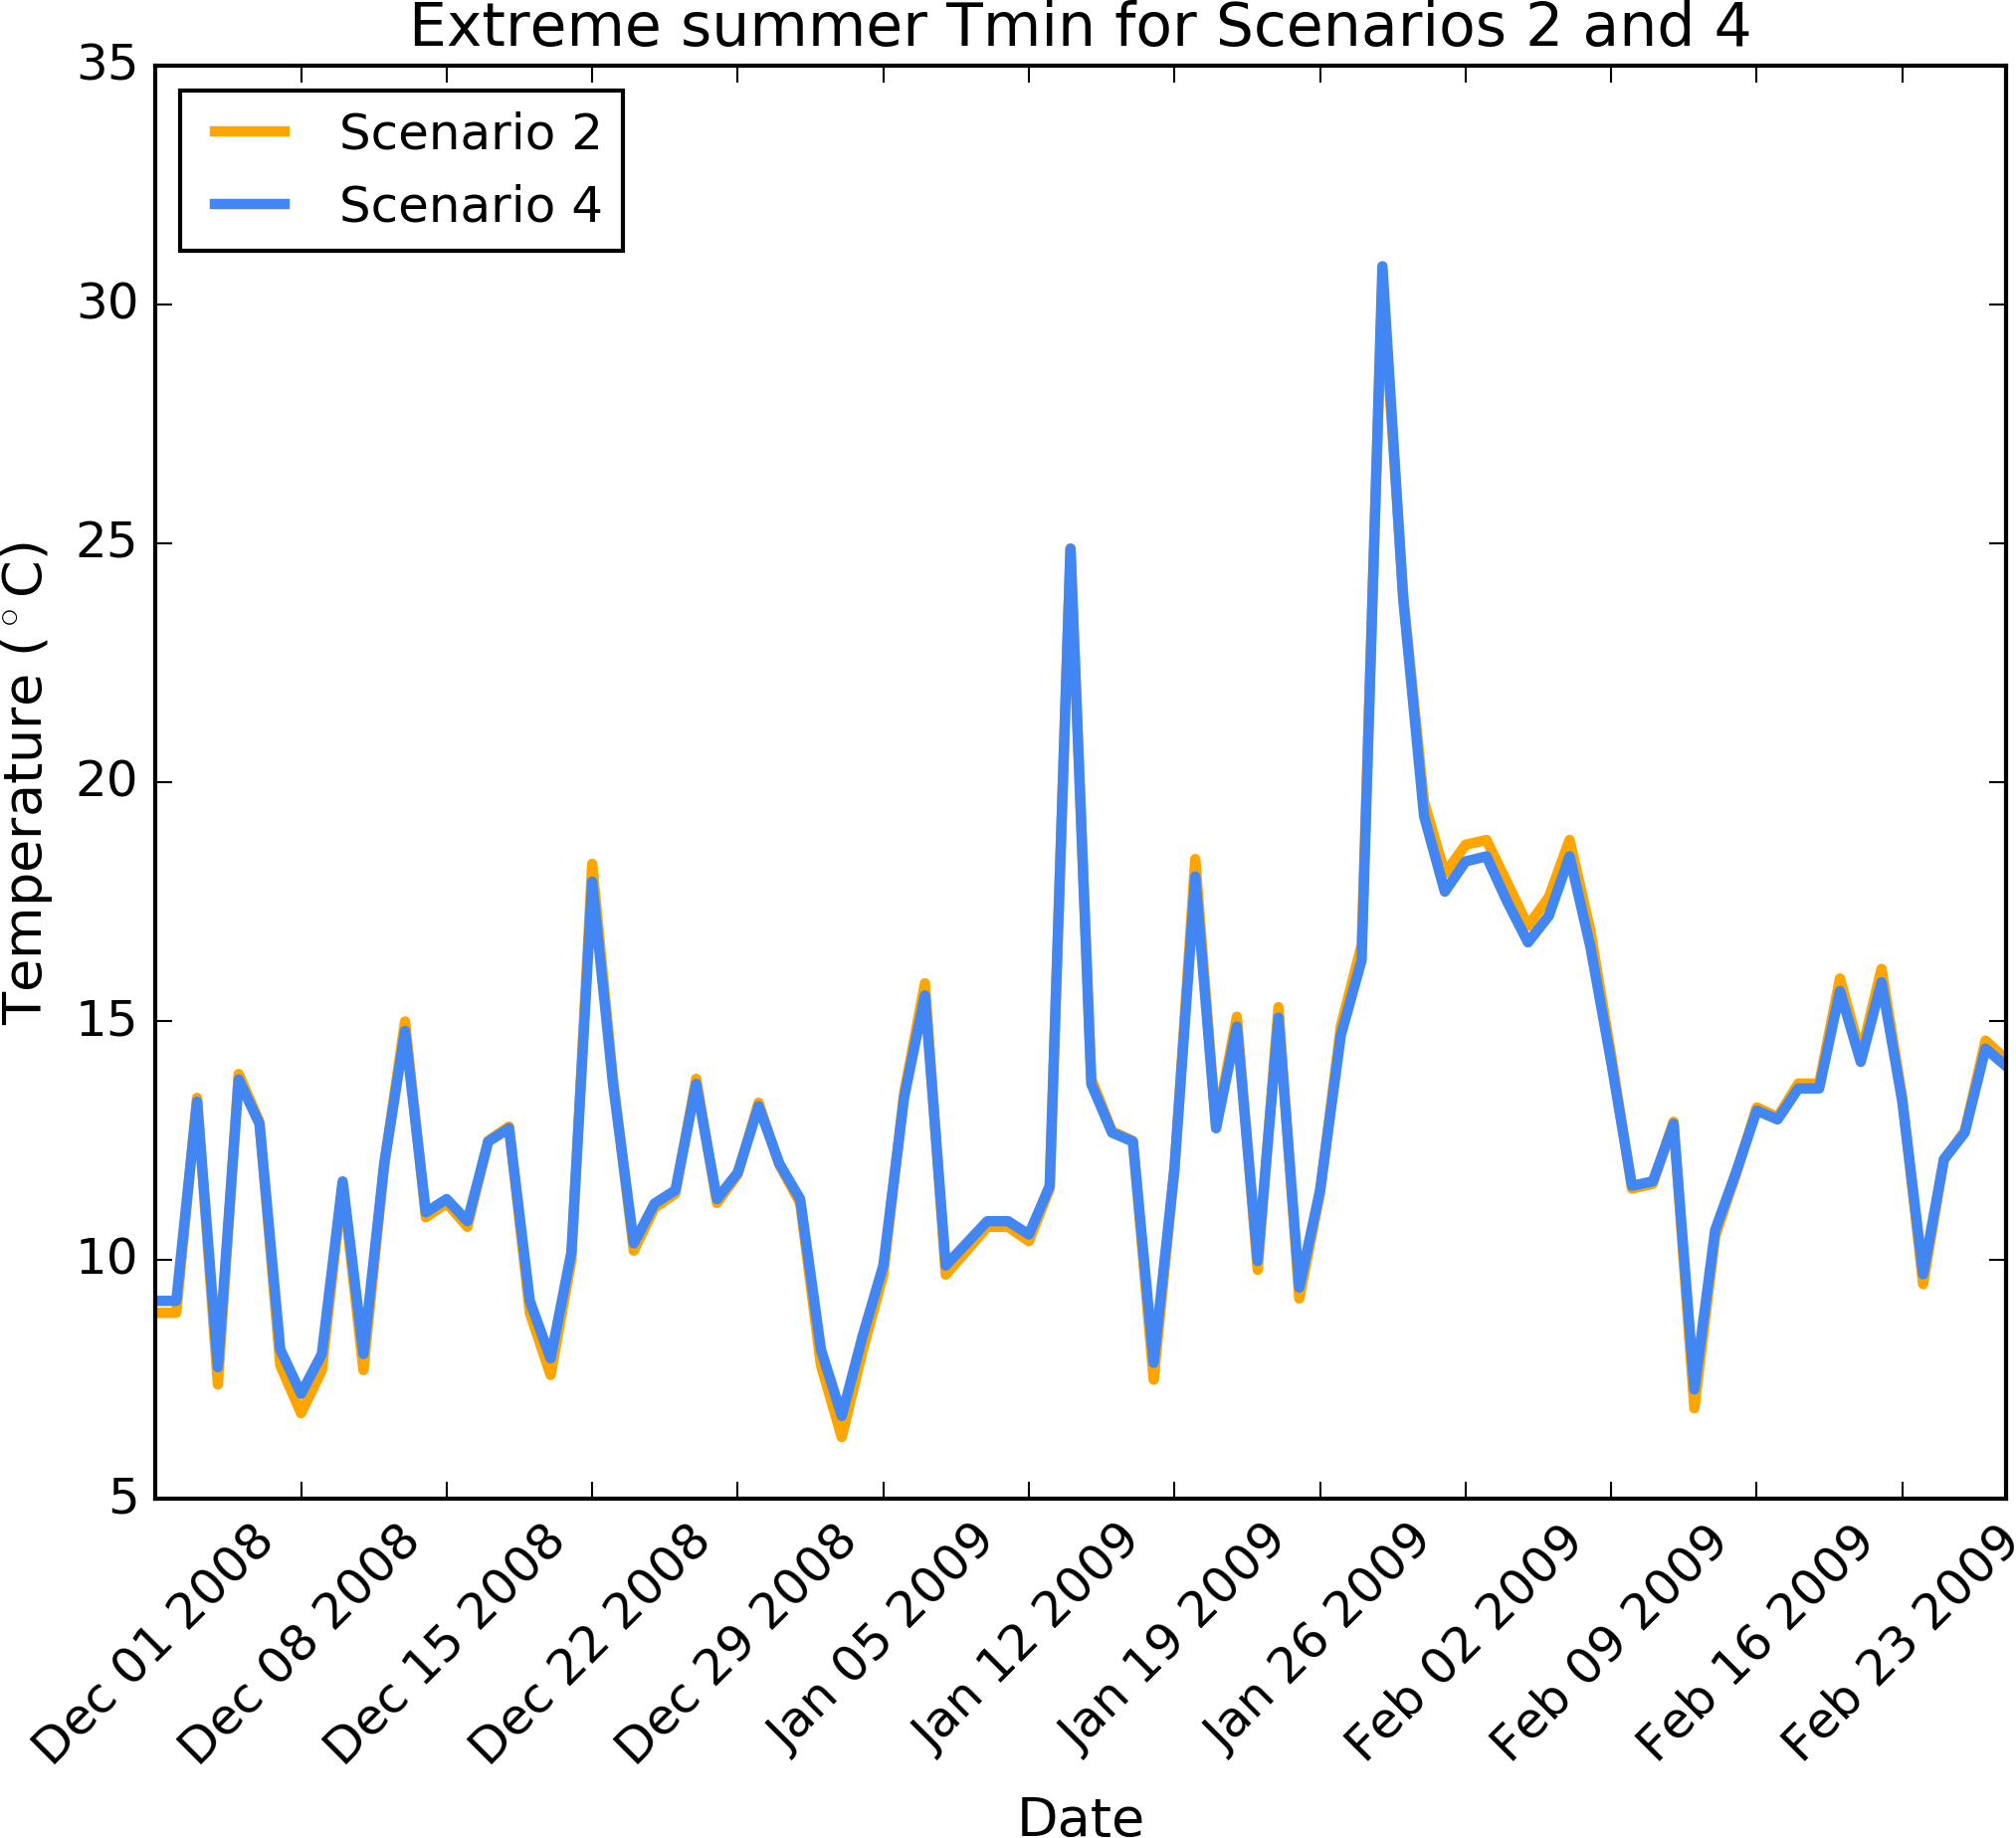
\includegraphics[scale=0.40]{images/fig5b} 
%\caption{\bf The observational (Scenario 2) and the WSUD Scenario 4 temperature mapped using linear interpolation for the (a) maximum and (b) minimum temperature. The two purple boxes indicate the January 28-30 2009 heatwave and the February 7 2009 Black Saturday event.}    
% \label{fig:fig5} 
%\end{figure} 



\section{Discussion}\label{sec:discussion}

\section{Conclusion}\label{sec:conclusion}





\section{Code availability}\label{sec:available}

\printglossary[title={List of Symbols}]

\section*{Acknowledgements}
The support of the Commonwealth of Australia through the Cooperative Research Centre program is acknowledged.
%\end{acknowledgements}

\section*{References}\label{sec:ref}
%% If you have bibdatabase file and want bibtex to generate the
%% bibitems, please use
%%
  \bibliographystyle{elsarticle-harv} 
  \bibliography{library}

%% else use the following coding to input the bibitems directly in the
%% TeX file.

\begin{thebibliography}{00}

%% \bibitem[Author(year)]{label}
%% Text of bibliographic item

\bibitem[ ()]{}

\end{thebibliography}


%% The Appendices part is started with the command \appendix;
%% appendix sections are then done as normal sections
%\appendix
%\setcounter{table}{0}
%\renewcommand{\thetable}{A\arabic{table}}

%\subsection{}                               %% Appendix A1, A2, etc.


%%%%%%%%%% taking out parameterizations
%\section{Appendix}\label{sec:app}  
%\subsection{Additional data tables}\label{app:tables}  




%\authorcontribution{This work was developed by Kerry Nice and supervised by Andrew Coutts and Nigel Tapper. Model source code was received from Scott Krayenhoff and Remko Duursma (as acknowledged in Section \ref{sec:available}). Synthesis of this code and new code was developed by Kerry Nice. The article was written by Kerry Nice with editing and suggestions from Andrew Coutts and Nigel Tapper.}
%
%\begin{acknowledgements}
%The work described in this paper was developed during a PhD. project at Monash University. Funding for this was obtailed through the City of Melbourne, Monash University, and the CRC for Water Sensitive Cities.  
%\end{acknowledgements}

%\begin{acknowledgements}
%The support of the Commonwealth of Australia through the Cooperative Research Centre program is acknowledged.
%\end{acknowledgements}






\end{document}

\endinput
%%
%% End of file `elsarticle-template-harv.tex'.
